\documentclass[twoside]{book}

% Packages required by doxygen
\usepackage{calc}
\usepackage{doxygen}
\usepackage{graphicx}
\usepackage[utf8]{inputenc}
\usepackage{makeidx}
\usepackage{multicol}
\usepackage{multirow}
\usepackage{textcomp}
\usepackage[table]{xcolor}

% Font selection
\usepackage[T1]{fontenc}
\usepackage{mathptmx}
\usepackage[scaled=.90]{helvet}
\usepackage{courier}
\usepackage{amssymb}
\usepackage{sectsty}
\renewcommand{\familydefault}{\sfdefault}
\allsectionsfont{%
  \fontseries{bc}\selectfont%
  \color{darkgray}%
}
\renewcommand{\DoxyLabelFont}{%
  \fontseries{bc}\selectfont%
  \color{darkgray}%
}

% Page & text layout
\usepackage{geometry}
\geometry{%
  a4paper,%
  top=2.5cm,%
  bottom=2.5cm,%
  left=2.5cm,%
  right=2.5cm%
}
\tolerance=750
\hfuzz=15pt
\hbadness=750
\setlength{\emergencystretch}{15pt}
\setlength{\parindent}{0cm}
\setlength{\parskip}{0.2cm}
\makeatletter
\renewcommand{\paragraph}{%
  \@startsection{paragraph}{4}{0ex}{-1.0ex}{1.0ex}{%
    \normalfont\normalsize\bfseries\SS@parafont%
  }%
}
\renewcommand{\subparagraph}{%
  \@startsection{subparagraph}{5}{0ex}{-1.0ex}{1.0ex}{%
    \normalfont\normalsize\bfseries\SS@subparafont%
  }%
}
\makeatother

% Headers & footers
\usepackage{fancyhdr}
\pagestyle{fancyplain}
\fancyhead[LE]{\fancyplain{}{\bfseries\thepage}}
\fancyhead[CE]{\fancyplain{}{}}
\fancyhead[RE]{\fancyplain{}{\bfseries\leftmark}}
\fancyhead[LO]{\fancyplain{}{\bfseries\rightmark}}
\fancyhead[CO]{\fancyplain{}{}}
\fancyhead[RO]{\fancyplain{}{\bfseries\thepage}}
\fancyfoot[LE]{\fancyplain{}{}}
\fancyfoot[CE]{\fancyplain{}{}}
\fancyfoot[RE]{\fancyplain{}{\bfseries\scriptsize Generated on Tue Mar 10 2015 16\-:54\-:19 for Justine -\/ a rapid prototype for development of G\-N\-U Robocar City Emulator and Robocar World Championship by Doxygen }}
\fancyfoot[LO]{\fancyplain{}{\bfseries\scriptsize Generated on Tue Mar 10 2015 16\-:54\-:19 for Justine -\/ a rapid prototype for development of G\-N\-U Robocar City Emulator and Robocar World Championship by Doxygen }}
\fancyfoot[CO]{\fancyplain{}{}}
\fancyfoot[RO]{\fancyplain{}{}}
\renewcommand{\footrulewidth}{0.4pt}
\renewcommand{\chaptermark}[1]{%
  \markboth{#1}{}%
}
\renewcommand{\sectionmark}[1]{%
  \markright{\thesection\ #1}%
}

% Indices & bibliography
\usepackage{natbib}
\usepackage[titles]{tocloft}
\setcounter{tocdepth}{3}
\setcounter{secnumdepth}{5}
\makeindex

% Hyperlinks (required, but should be loaded last)
\usepackage{ifpdf}
\ifpdf
  \usepackage[pdftex,pagebackref=true]{hyperref}
\else
  \usepackage[ps2pdf,pagebackref=true]{hyperref}
\fi
\hypersetup{%
  colorlinks=true,%
  linkcolor=blue,%
  citecolor=blue,%
  unicode%
}

% Custom commands
\newcommand{\clearemptydoublepage}{%
  \newpage{\pagestyle{empty}\cleardoublepage}%
}


%===== C O N T E N T S =====

\begin{document}

% Titlepage & ToC
\hypersetup{pageanchor=false}
\pagenumbering{roman}
\begin{titlepage}
\vspace*{7cm}
\begin{center}%
{\Large Justine -\/ a rapid prototype for development of G\-N\-U Robocar City Emulator and Robocar World Championship \\[1ex]\large 0.\-0.\-12 }\\
\vspace*{1cm}
{\large Generated by Doxygen 1.8.6}\\
\vspace*{0.5cm}
{\small Tue Mar 10 2015 16:54:19}\\
\end{center}
\end{titlepage}
\clearemptydoublepage
\tableofcontents
\clearemptydoublepage
\pagenumbering{arabic}
\hypersetup{pageanchor=true}

%--- Begin generated contents ---
\chapter{Justine -\/ this is a rapid prototype for development of Robocar City Emulator}
\label{index}\hypertarget{index}{}\begin{DoxyAuthor}{Authors}
Norbert Bátfai \href{mailto:nbatfai@gmail.com}{\tt nbatfai@gmail.\-com}
\end{DoxyAuthor}
\hypertarget{index_intro}{}\section{Introduction}\label{index_intro}

\chapter{Hierarchical Index}
\section{Class Hierarchy}
This inheritance list is sorted roughly, but not completely, alphabetically\-:\begin{DoxyCompactList}
\item \contentsline{section}{justine\-:\-:robocar\-:\-:Car}{\pageref{classjustine_1_1robocar_1_1Car}}{}
\begin{DoxyCompactList}
\item \contentsline{section}{justine\-:\-:robocar\-:\-:Ant\-Car}{\pageref{classjustine_1_1robocar_1_1AntCar}}{}
\item \contentsline{section}{justine\-:\-:robocar\-:\-:Smart\-Car}{\pageref{classjustine_1_1robocar_1_1SmartCar}}{}
\begin{DoxyCompactList}
\item \contentsline{section}{justine\-:\-:robocar\-:\-:Cop\-Car}{\pageref{classjustine_1_1robocar_1_1CopCar}}{}
\end{DoxyCompactList}
\end{DoxyCompactList}
\item Handler\begin{DoxyCompactList}
\item \contentsline{section}{justine\-:\-:robocar\-:\-:O\-S\-M\-Reader}{\pageref{classjustine_1_1robocar_1_1OSMReader}}{}
\end{DoxyCompactList}
\item \contentsline{section}{justine\-:\-:robocar\-:\-:Shared\-Data}{\pageref{classjustine_1_1robocar_1_1SharedData}}{}
\item \contentsline{section}{justine\-:\-:sampleclient\-:\-:Shm\-Client}{\pageref{classjustine_1_1sampleclient_1_1ShmClient}}{}
\begin{DoxyCompactList}
\item \contentsline{section}{justine\-:\-:sampleclient\-:\-:My\-Shm\-Client}{\pageref{classjustine_1_1sampleclient_1_1MyShmClient}}{}
\end{DoxyCompactList}
\item \contentsline{section}{justine\-:\-:robocar\-:\-:Smart\-City}{\pageref{classjustine_1_1robocar_1_1SmartCity}}{}
\item \contentsline{section}{justine\-:\-:robocar\-:\-:Traffic}{\pageref{classjustine_1_1robocar_1_1Traffic}}{}
\item \contentsline{section}{yy\-\_\-buffer\-\_\-state}{\pageref{structyy__buffer__state}}{}
\item \contentsline{section}{yy\-\_\-trans\-\_\-info}{\pageref{structyy__trans__info}}{}
\item yy\-Flex\-Lexer\begin{DoxyCompactList}
\item \contentsline{section}{justine\-:\-:robocar\-:\-:Car\-Lexer}{\pageref{classjustine_1_1robocar_1_1CarLexer}}{}
\end{DoxyCompactList}
\end{DoxyCompactList}

\chapter{Class Index}
\section{Class List}
Here are the classes, structs, unions and interfaces with brief descriptions\-:\begin{DoxyCompactList}
\item\contentsline{section}{\hyperlink{classjustine_1_1robocar_1_1AntCar}{justine\-::robocar\-::\-Ant\-Car} }{\pageref{classjustine_1_1robocar_1_1AntCar}}{}
\item\contentsline{section}{\hyperlink{classjustine_1_1robocar_1_1Car}{justine\-::robocar\-::\-Car} }{\pageref{classjustine_1_1robocar_1_1Car}}{}
\item\contentsline{section}{\hyperlink{classjustine_1_1robocar_1_1CarLexer}{justine\-::robocar\-::\-Car\-Lexer} }{\pageref{classjustine_1_1robocar_1_1CarLexer}}{}
\item\contentsline{section}{\hyperlink{classjustine_1_1robocar_1_1CopCar}{justine\-::robocar\-::\-Cop\-Car} }{\pageref{classjustine_1_1robocar_1_1CopCar}}{}
\item\contentsline{section}{\hyperlink{classjustine_1_1sampleclient_1_1MyShmClient}{justine\-::sampleclient\-::\-My\-Shm\-Client} \\*A sample class used for testing the routing algorithms }{\pageref{classjustine_1_1sampleclient_1_1MyShmClient}}{}
\item\contentsline{section}{\hyperlink{classjustine_1_1robocar_1_1OSMReader}{justine\-::robocar\-::\-O\-S\-M\-Reader} }{\pageref{classjustine_1_1robocar_1_1OSMReader}}{}
\item\contentsline{section}{\hyperlink{classjustine_1_1robocar_1_1SharedData}{justine\-::robocar\-::\-Shared\-Data} }{\pageref{classjustine_1_1robocar_1_1SharedData}}{}
\item\contentsline{section}{\hyperlink{classjustine_1_1sampleclient_1_1ShmClient}{justine\-::sampleclient\-::\-Shm\-Client} \\*A sample class used for testing I\-P\-C mechanisms (S\-H\-M and sockets) which are used by the city emulator }{\pageref{classjustine_1_1sampleclient_1_1ShmClient}}{}
\item\contentsline{section}{\hyperlink{classjustine_1_1robocar_1_1SmartCar}{justine\-::robocar\-::\-Smart\-Car} }{\pageref{classjustine_1_1robocar_1_1SmartCar}}{}
\item\contentsline{section}{\hyperlink{classjustine_1_1robocar_1_1SmartCity}{justine\-::robocar\-::\-Smart\-City} }{\pageref{classjustine_1_1robocar_1_1SmartCity}}{}
\item\contentsline{section}{\hyperlink{classjustine_1_1robocar_1_1Traffic}{justine\-::robocar\-::\-Traffic} }{\pageref{classjustine_1_1robocar_1_1Traffic}}{}
\item\contentsline{section}{\hyperlink{structyy__buffer__state}{yy\-\_\-buffer\-\_\-state} }{\pageref{structyy__buffer__state}}{}
\item\contentsline{section}{\hyperlink{structyy__trans__info}{yy\-\_\-trans\-\_\-info} }{\pageref{structyy__trans__info}}{}
\end{DoxyCompactList}

\chapter{File Index}
\section{File List}
Here is a list of all documented files with brief descriptions\-:\begin{DoxyCompactList}
\item\contentsline{section}{src/\hyperlink{car_8cpp}{car.\-cpp} \\*Justine -\/ this is a rapid prototype for development of Robocar City Emulator }{\pageref{car_8cpp}}{}
\item\contentsline{section}{src/\hyperlink{car_8hpp}{car.\-hpp} \\*Justine -\/ this is a rapid prototype for development of Robocar City Emulator }{\pageref{car_8hpp}}{}
\item\contentsline{section}{src/{\bfseries carlexer.\-cc} }{\pageref{carlexer_8cc}}{}
\item\contentsline{section}{src/\hyperlink{carlexer_8hpp}{carlexer.\-hpp} \\*Justine -\/ this is a rapid prototype for development of Robocar City Emulator }{\pageref{carlexer_8hpp}}{}
\item\contentsline{section}{src/\hyperlink{mainpage_8h}{mainpage.\-h} \\*Justine -\/ this is a rapid prototype for development of Robocar City Emulator }{\pageref{mainpage_8h}}{}
\item\contentsline{section}{src/\hyperlink{myshmclient-main_8cpp}{myshmclient-\/main.\-cpp} \\*Justine -\/ this is a rapid prototype for development of Robocar City Emulator }{\pageref{myshmclient-main_8cpp}}{}
\item\contentsline{section}{src/\hyperlink{myshmclient_8cpp}{myshmclient.\-cpp} \\*Justine -\/ this is a rapid prototype for development of Robocar City Emulator }{\pageref{myshmclient_8cpp}}{}
\item\contentsline{section}{src/\hyperlink{myshmclient_8hpp}{myshmclient.\-hpp} \\*Justine -\/ this is a rapid prototype for development of Robocar City Emulator }{\pageref{myshmclient_8hpp}}{}
\item\contentsline{section}{src/\hyperlink{osmreader_8hpp}{osmreader.\-hpp} \\*Justine -\/ this is a rapid prototype for development of Robocar City Emulator }{\pageref{osmreader_8hpp}}{}
\item\contentsline{section}{src/\hyperlink{shmclient-main_8cpp}{shmclient-\/main.\-cpp} \\*Justine -\/ this is a rapid prototype for development of Robocar City Emulator }{\pageref{shmclient-main_8cpp}}{}
\item\contentsline{section}{src/\hyperlink{shmclient_8cpp}{shmclient.\-cpp} \\*Justine -\/ this is a rapid prototype for development of Robocar City Emulator }{\pageref{shmclient_8cpp}}{}
\item\contentsline{section}{src/\hyperlink{shmclient_8hpp}{shmclient.\-hpp} \\*Justine -\/ this is a rapid prototype for development of Robocar City Emulator }{\pageref{shmclient_8hpp}}{}
\item\contentsline{section}{src/{\bfseries smartcity.\-cpp} }{\pageref{smartcity_8cpp}}{}
\item\contentsline{section}{src/\hyperlink{smartcity_8hpp}{smartcity.\-hpp} \\*Justine -\/ this is a rapid prototype for development of Robocar City Emulator }{\pageref{smartcity_8hpp}}{}
\item\contentsline{section}{src/\hyperlink{traffic-main_8cpp}{traffic-\/main.\-cpp} \\*Justine -\/ this is a rapid prototype for development of Robocar City Emulator }{\pageref{traffic-main_8cpp}}{}
\item\contentsline{section}{src/\hyperlink{traffic_8cpp}{traffic.\-cpp} \\*Justine -\/ this is a rapid prototype for development of Robocar City Emulator }{\pageref{traffic_8cpp}}{}
\item\contentsline{section}{src/{\bfseries traffic.\-hpp} }{\pageref{traffic_8hpp}}{}
\end{DoxyCompactList}

\chapter{Class Documentation}
\hypertarget{classjustine_1_1robocar_1_1AntCar}{\section{justine\-:\-:robocar\-:\-:Ant\-Car Class Reference}
\label{classjustine_1_1robocar_1_1AntCar}\index{justine\-::robocar\-::\-Ant\-Car@{justine\-::robocar\-::\-Ant\-Car}}
}
Inheritance diagram for justine\-:\-:robocar\-:\-:Ant\-Car\-:\begin{figure}[H]
\begin{center}
\leavevmode
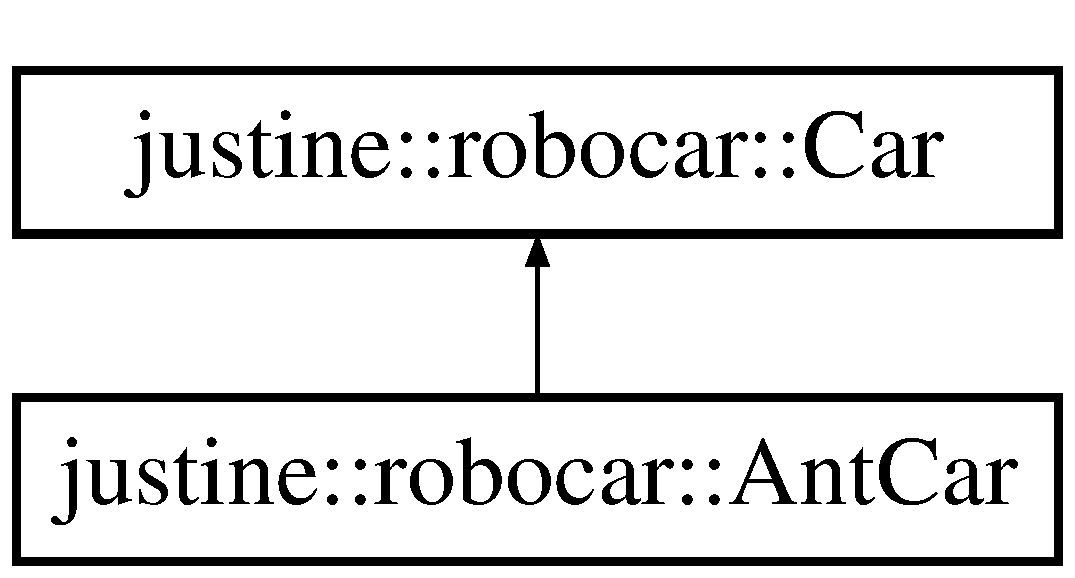
\includegraphics[height=2.000000cm]{classjustine_1_1robocar_1_1AntCar}
\end{center}
\end{figure}
\subsection*{Public Member Functions}
\begin{DoxyCompactItemize}
\item 
\hypertarget{classjustine_1_1robocar_1_1AntCar_ad6d3febd3d0c0bd2741f0c9e88699b71}{{\bfseries Ant\-Car} (\hyperlink{classjustine_1_1robocar_1_1Traffic}{Traffic} \&traffic)}\label{classjustine_1_1robocar_1_1AntCar_ad6d3febd3d0c0bd2741f0c9e88699b71}

\item 
\hypertarget{classjustine_1_1robocar_1_1AntCar_a09670994e3ad6d71a09bf270c6b14546}{virtual void {\bfseries next\-Smarter\-Edge} (void)}\label{classjustine_1_1robocar_1_1AntCar_a09670994e3ad6d71a09bf270c6b14546}

\item 
\hypertarget{classjustine_1_1robocar_1_1AntCar_a5d792cb28b1746420870d683f7cd46be}{virtual void {\bfseries print} (std\-::ostream \&os) const }\label{classjustine_1_1robocar_1_1AntCar_a5d792cb28b1746420870d683f7cd46be}

\item 
\hypertarget{classjustine_1_1robocar_1_1AntCar_aa4b9814ad0c29c66f9206d46b517058c}{osmium\-::unsigned\-\_\-object\-\_\-id\-\_\-type {\bfseries ant} (void)}\label{classjustine_1_1robocar_1_1AntCar_aa4b9814ad0c29c66f9206d46b517058c}

\item 
\hypertarget{classjustine_1_1robocar_1_1AntCar_a364d9699615685f3167a718497da6ef8}{osmium\-::unsigned\-\_\-object\-\_\-id\-\_\-type {\bfseries ant\-\_\-rnd} (void)}\label{classjustine_1_1robocar_1_1AntCar_a364d9699615685f3167a718497da6ef8}

\item 
\hypertarget{classjustine_1_1robocar_1_1AntCar_a2f61c529a99befbc6404e7755ea07afe}{osmium\-::unsigned\-\_\-object\-\_\-id\-\_\-type {\bfseries ant\-\_\-rernd} (void)}\label{classjustine_1_1robocar_1_1AntCar_a2f61c529a99befbc6404e7755ea07afe}

\item 
\hypertarget{classjustine_1_1robocar_1_1AntCar_a86068ebe62971609c3dcd75fb7510497}{osmium\-::unsigned\-\_\-object\-\_\-id\-\_\-type {\bfseries ant\-\_\-mrernd} (void)}\label{classjustine_1_1robocar_1_1AntCar_a86068ebe62971609c3dcd75fb7510497}

\end{DoxyCompactItemize}
\subsection*{Static Public Attributes}
\begin{DoxyCompactItemize}
\item 
\hypertarget{classjustine_1_1robocar_1_1AntCar_a2d1809d2478876a8dff4fffe1632aebd}{static Adjacency\-List {\bfseries alist}}\label{classjustine_1_1robocar_1_1AntCar_a2d1809d2478876a8dff4fffe1632aebd}

\item 
\hypertarget{classjustine_1_1robocar_1_1AntCar_a2b945e75caa713e5276908ace9fe3a7c}{static Adjacency\-List {\bfseries alist\-\_\-evaporate}}\label{classjustine_1_1robocar_1_1AntCar_a2b945e75caa713e5276908ace9fe3a7c}

\end{DoxyCompactItemize}
\subsection*{Additional Inherited Members}


\subsection{Detailed Description}


Definition at line 126 of file car.\-hpp.



The documentation for this class was generated from the following files\-:\begin{DoxyCompactItemize}
\item 
src/\hyperlink{car_8hpp}{car.\-hpp}\item 
src/\hyperlink{car_8cpp}{car.\-cpp}\end{DoxyCompactItemize}

\hypertarget{classjustine_1_1robocar_1_1Car}{\section{justine\-:\-:robocar\-:\-:Car Class Reference}
\label{classjustine_1_1robocar_1_1Car}\index{justine\-::robocar\-::\-Car@{justine\-::robocar\-::\-Car}}
}
Inheritance diagram for justine\-:\-:robocar\-:\-:Car\-:\begin{figure}[H]
\begin{center}
\leavevmode
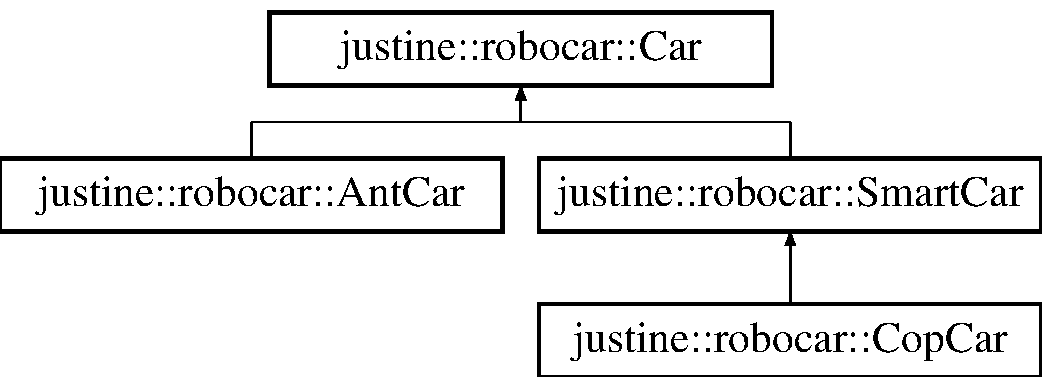
\includegraphics[height=3.000000cm]{classjustine_1_1robocar_1_1Car}
\end{center}
\end{figure}
\subsection*{Public Member Functions}
\begin{DoxyCompactItemize}
\item 
\hypertarget{classjustine_1_1robocar_1_1Car_ae3cb19dcf6cbee13fa22247dfbe857d7}{{\bfseries Car} (\hyperlink{classjustine_1_1robocar_1_1Traffic}{Traffic} \&traffic, Car\-Type type=Car\-Type\-::\-N\-O\-R\-M\-A\-L)}\label{classjustine_1_1robocar_1_1Car_ae3cb19dcf6cbee13fa22247dfbe857d7}

\item 
\hypertarget{classjustine_1_1robocar_1_1Car_a6448560523b0271b86be67e3e6505f4a}{virtual void {\bfseries init} ()}\label{classjustine_1_1robocar_1_1Car_a6448560523b0271b86be67e3e6505f4a}

\item 
\hypertarget{classjustine_1_1robocar_1_1Car_a8714ac61dc6eb8ad2baef998aa6e8758}{virtual void {\bfseries step} ()}\label{classjustine_1_1robocar_1_1Car_a8714ac61dc6eb8ad2baef998aa6e8758}

\item 
\hypertarget{classjustine_1_1robocar_1_1Car_a6f687cc942b9703896e4611dcd0de687}{osmium\-::unsigned\-\_\-object\-\_\-id\-\_\-type {\bfseries from} () const }\label{classjustine_1_1robocar_1_1Car_a6f687cc942b9703896e4611dcd0de687}

\item 
\hypertarget{classjustine_1_1robocar_1_1Car_a089017383dbbe588dd1235bee18b3be1}{osmium\-::unsigned\-\_\-object\-\_\-id\-\_\-type {\bfseries to} () const }\label{classjustine_1_1robocar_1_1Car_a089017383dbbe588dd1235bee18b3be1}

\item 
\hypertarget{classjustine_1_1robocar_1_1Car_ada98233230a5f4acc9dcabccc17f9d9c}{osmium\-::unsigned\-\_\-object\-\_\-id\-\_\-type {\bfseries get\-\_\-step} () const }\label{classjustine_1_1robocar_1_1Car_ada98233230a5f4acc9dcabccc17f9d9c}

\item 
\hypertarget{classjustine_1_1robocar_1_1Car_a6ea284ecb2413f121092f925ca9275fc}{Car\-Type {\bfseries get\-\_\-type} () const }\label{classjustine_1_1robocar_1_1Car_a6ea284ecb2413f121092f925ca9275fc}

\item 
\hypertarget{classjustine_1_1robocar_1_1Car_a00607bcb72a39b4188f80ecb384e0014}{void {\bfseries set\-\_\-type} (Car\-Type type)}\label{classjustine_1_1robocar_1_1Car_a00607bcb72a39b4188f80ecb384e0014}

\item 
\hypertarget{classjustine_1_1robocar_1_1Car_aad2ce1d99d84215f9d963576d89cd777}{osmium\-::unsigned\-\_\-object\-\_\-id\-\_\-type {\bfseries to\-\_\-node} () const }\label{classjustine_1_1robocar_1_1Car_aad2ce1d99d84215f9d963576d89cd777}

\item 
\hypertarget{classjustine_1_1robocar_1_1Car_a02ff825fb44880bb7130ad1721398b27}{osmium\-::unsigned\-\_\-object\-\_\-id\-\_\-type {\bfseries get\-\_\-max\-\_\-steps} () const }\label{classjustine_1_1robocar_1_1Car_a02ff825fb44880bb7130ad1721398b27}

\item 
\hypertarget{classjustine_1_1robocar_1_1Car_a0fae4d710d8337ec1df25f00341c4e9c}{virtual void {\bfseries next\-Edge} (void)}\label{classjustine_1_1robocar_1_1Car_a0fae4d710d8337ec1df25f00341c4e9c}

\item 
\hypertarget{classjustine_1_1robocar_1_1Car_a3e0ac48e03b4307cc200d5b6a7ff7653}{virtual void {\bfseries next\-Smarter\-Edge} (void)}\label{classjustine_1_1robocar_1_1Car_a3e0ac48e03b4307cc200d5b6a7ff7653}

\item 
\hypertarget{classjustine_1_1robocar_1_1Car_a71649d538dfafc0e850fe782c55a173e}{virtual void {\bfseries print} (std\-::ostream \&os) const }\label{classjustine_1_1robocar_1_1Car_a71649d538dfafc0e850fe782c55a173e}

\end{DoxyCompactItemize}
\subsection*{Protected Attributes}
\begin{DoxyCompactItemize}
\item 
\hypertarget{classjustine_1_1robocar_1_1Car_a4f99adee89f8a1ca91f6fc030c97feca}{\hyperlink{classjustine_1_1robocar_1_1Traffic}{Traffic} \& {\bfseries traffic}}\label{classjustine_1_1robocar_1_1Car_a4f99adee89f8a1ca91f6fc030c97feca}

\item 
\hypertarget{classjustine_1_1robocar_1_1Car_ad155992312519e7fba23bdd860d615a8}{Car\-Type {\bfseries m\-\_\-type} \{Car\-Type\-::\-N\-O\-R\-M\-A\-L\}}\label{classjustine_1_1robocar_1_1Car_ad155992312519e7fba23bdd860d615a8}

\item 
\hypertarget{classjustine_1_1robocar_1_1Car_a0858b48ca22e62eaf8a7c36dc2c9705f}{osmium\-::unsigned\-\_\-object\-\_\-id\-\_\-type {\bfseries m\-\_\-from} \{3130863972\}}\label{classjustine_1_1robocar_1_1Car_a0858b48ca22e62eaf8a7c36dc2c9705f}

\item 
\hypertarget{classjustine_1_1robocar_1_1Car_a78c32854d0f75624343af5cba33fc725}{osmium\-::unsigned\-\_\-object\-\_\-id\-\_\-type {\bfseries m\-\_\-to} \{0\}}\label{classjustine_1_1robocar_1_1Car_a78c32854d0f75624343af5cba33fc725}

\item 
\hypertarget{classjustine_1_1robocar_1_1Car_ad1ea1c329f34b6f8e51f19067911201a}{osmium\-::unsigned\-\_\-object\-\_\-id\-\_\-type {\bfseries m\-\_\-step} \{0\}}\label{classjustine_1_1robocar_1_1Car_ad1ea1c329f34b6f8e51f19067911201a}

\end{DoxyCompactItemize}
\subsection*{Friends}
\begin{DoxyCompactItemize}
\item 
\hypertarget{classjustine_1_1robocar_1_1Car_a6d89810a4431b2bdbeeb0c9f31fee556}{std\-::ostream \& {\bfseries operator$<$$<$} (std\-::ostream \&os, \hyperlink{classjustine_1_1robocar_1_1Car}{Car} \&c)}\label{classjustine_1_1robocar_1_1Car_a6d89810a4431b2bdbeeb0c9f31fee556}

\end{DoxyCompactItemize}


\subsection{Detailed Description}


Definition at line 55 of file car.\-hpp.



The documentation for this class was generated from the following files\-:\begin{DoxyCompactItemize}
\item 
src/\hyperlink{car_8hpp}{car.\-hpp}\item 
src/\hyperlink{car_8cpp}{car.\-cpp}\end{DoxyCompactItemize}

\hypertarget{classjustine_1_1robocar_1_1CarLexer}{\section{justine\-:\-:robocar\-:\-:Car\-Lexer Class Reference}
\label{classjustine_1_1robocar_1_1CarLexer}\index{justine\-::robocar\-::\-Car\-Lexer@{justine\-::robocar\-::\-Car\-Lexer}}
}
Inheritance diagram for justine\-:\-:robocar\-:\-:Car\-Lexer\-:\begin{figure}[H]
\begin{center}
\leavevmode
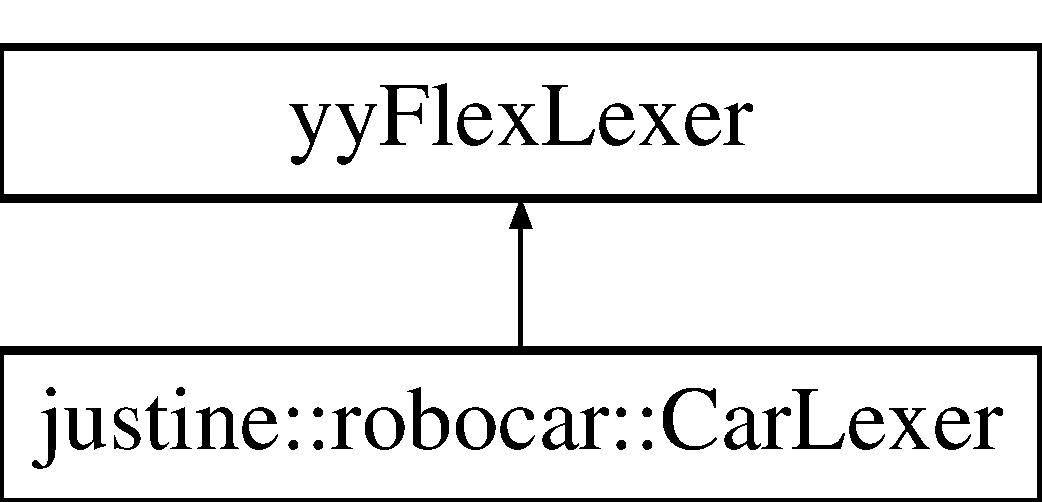
\includegraphics[height=2.000000cm]{classjustine_1_1robocar_1_1CarLexer}
\end{center}
\end{figure}
\subsection*{Public Member Functions}
\begin{DoxyCompactItemize}
\item 
\hypertarget{classjustine_1_1robocar_1_1CarLexer_a141ae0c2aa9fb37b6045f4126377aa4e}{virtual int {\bfseries yylex} ()}\label{classjustine_1_1robocar_1_1CarLexer_a141ae0c2aa9fb37b6045f4126377aa4e}

\item 
\hypertarget{classjustine_1_1robocar_1_1CarLexer_a64216c04da2303504e4761b8b1f3cbd7}{char $\ast$ {\bfseries get\-\_\-name} ()}\label{classjustine_1_1robocar_1_1CarLexer_a64216c04da2303504e4761b8b1f3cbd7}

\item 
\hypertarget{classjustine_1_1robocar_1_1CarLexer_a5d7b64b987f72638492b5d7fb874e027}{char {\bfseries get\-\_\-role} () const }\label{classjustine_1_1robocar_1_1CarLexer_a5d7b64b987f72638492b5d7fb874e027}

\item 
\hypertarget{classjustine_1_1robocar_1_1CarLexer_a5f76db35df8712c3ca96941dea284261}{int {\bfseries get\-\_\-num} () const }\label{classjustine_1_1robocar_1_1CarLexer_a5f76db35df8712c3ca96941dea284261}

\item 
\hypertarget{classjustine_1_1robocar_1_1CarLexer_a2d033282421fefd97de5e527dd9098e1}{int {\bfseries get\-\_\-errnumber} () const }\label{classjustine_1_1robocar_1_1CarLexer_a2d033282421fefd97de5e527dd9098e1}

\item 
\hypertarget{classjustine_1_1robocar_1_1CarLexer_a32c2849b020dcc0d17f4d0b7c63e4bd4}{bool {\bfseries get\-\_\-guided} () const }\label{classjustine_1_1robocar_1_1CarLexer_a32c2849b020dcc0d17f4d0b7c63e4bd4}

\item 
\hypertarget{classjustine_1_1robocar_1_1CarLexer_a0f33aba8fabacd366d1cc5e1569de648}{int {\bfseries get\-\_\-cmd} () const }\label{classjustine_1_1robocar_1_1CarLexer_a0f33aba8fabacd366d1cc5e1569de648}

\item 
\hypertarget{classjustine_1_1robocar_1_1CarLexer_ab93d617ee8e18853ad555061af508259}{int {\bfseries get\-\_\-id} () const }\label{classjustine_1_1robocar_1_1CarLexer_ab93d617ee8e18853ad555061af508259}

\item 
\hypertarget{classjustine_1_1robocar_1_1CarLexer_a74023d4b3f9257dea8b65d9c65159c39}{std\-::vector$<$ unsigned int $>$ \& {\bfseries get\-\_\-route} (void)}\label{classjustine_1_1robocar_1_1CarLexer_a74023d4b3f9257dea8b65d9c65159c39}

\item 
\hypertarget{classjustine_1_1robocar_1_1CarLexer_a10ccec79e665a0fa52a3c53b30a0a76c}{unsigned int {\bfseries get\-\_\-from} () const }\label{classjustine_1_1robocar_1_1CarLexer_a10ccec79e665a0fa52a3c53b30a0a76c}

\item 
\hypertarget{classjustine_1_1robocar_1_1CarLexer_a8991b70b12f6db425c66f42bb5043418}{unsigned int {\bfseries get\-\_\-to} () const }\label{classjustine_1_1robocar_1_1CarLexer_a8991b70b12f6db425c66f42bb5043418}

\end{DoxyCompactItemize}
\subsection*{Friends}
\begin{DoxyCompactItemize}
\item 
\hypertarget{classjustine_1_1robocar_1_1CarLexer_ad3dfd377825cf79a0ef131deac8158c1}{std\-::ostream \& {\bfseries operator$<$$<$} (std\-::ostream \&os, \hyperlink{classjustine_1_1robocar_1_1CarLexer}{Car\-Lexer} \&cl)}\label{classjustine_1_1robocar_1_1CarLexer_ad3dfd377825cf79a0ef131deac8158c1}

\end{DoxyCompactItemize}


\subsection{Detailed Description}


Definition at line 50 of file carlexer.\-hpp.



The documentation for this class was generated from the following file\-:\begin{DoxyCompactItemize}
\item 
src/\hyperlink{carlexer_8hpp}{carlexer.\-hpp}\end{DoxyCompactItemize}

\hypertarget{classjustine_1_1robocar_1_1CopCar}{\section{justine\-:\-:robocar\-:\-:Cop\-Car Class Reference}
\label{classjustine_1_1robocar_1_1CopCar}\index{justine\-::robocar\-::\-Cop\-Car@{justine\-::robocar\-::\-Cop\-Car}}
}
Inheritance diagram for justine\-:\-:robocar\-:\-:Cop\-Car\-:\begin{figure}[H]
\begin{center}
\leavevmode
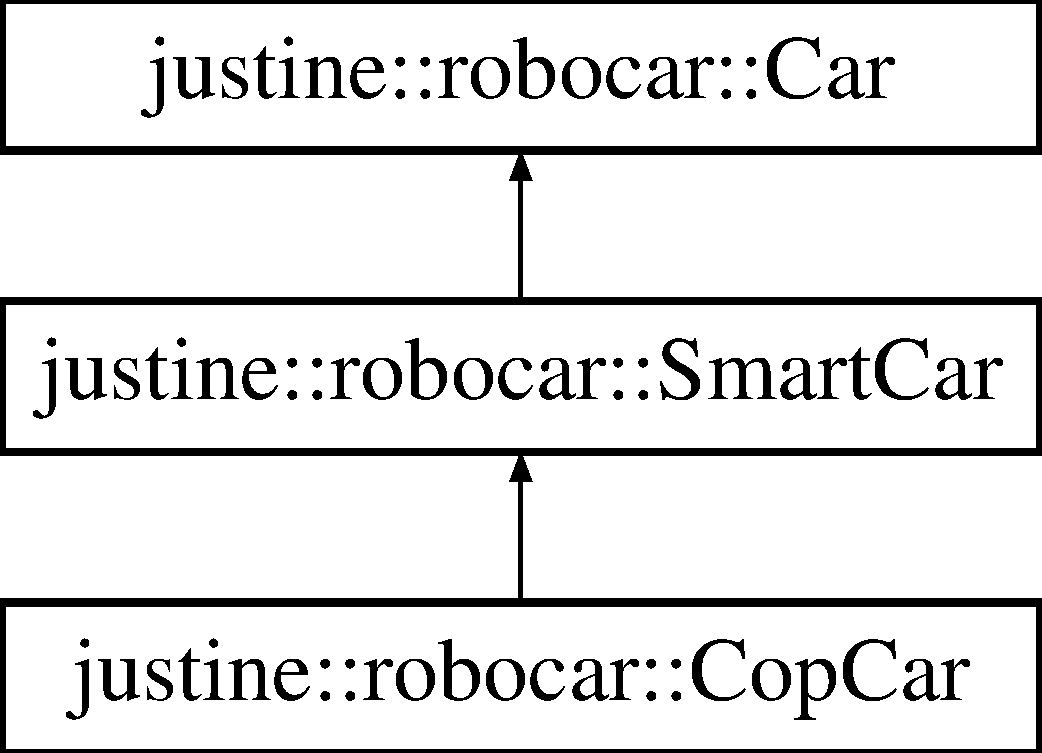
\includegraphics[height=3.000000cm]{classjustine_1_1robocar_1_1CopCar}
\end{center}
\end{figure}
\subsection*{Public Member Functions}
\begin{DoxyCompactItemize}
\item 
\hypertarget{classjustine_1_1robocar_1_1CopCar_a1fd71f225b51069993fa896387a0c3c6}{{\bfseries Cop\-Car} (\hyperlink{classjustine_1_1robocar_1_1Traffic}{Traffic} \&traffic, bool guided, const char $\ast$name)}\label{classjustine_1_1robocar_1_1CopCar_a1fd71f225b51069993fa896387a0c3c6}

\item 
\hypertarget{classjustine_1_1robocar_1_1CopCar_aa47580db59f0cb892d5649769de08999}{virtual void {\bfseries print} (std\-::ostream \&os) const }\label{classjustine_1_1robocar_1_1CopCar_aa47580db59f0cb892d5649769de08999}

\item 
\hypertarget{classjustine_1_1robocar_1_1CopCar_a3e008915c7295de23793f8bccad3ff4a}{std\-::string {\bfseries get\-\_\-name} () const }\label{classjustine_1_1robocar_1_1CopCar_a3e008915c7295de23793f8bccad3ff4a}

\item 
\hypertarget{classjustine_1_1robocar_1_1CopCar_a50060362f00b3a82bab7590350c5fbca}{int {\bfseries get\-\_\-num\-\_\-captured\-\_\-gangsters} () const }\label{classjustine_1_1robocar_1_1CopCar_a50060362f00b3a82bab7590350c5fbca}

\item 
\hypertarget{classjustine_1_1robocar_1_1CopCar_acc9888c1b4b288543ca3c4df9767d34f}{void {\bfseries captured\-\_\-gangster} (void)}\label{classjustine_1_1robocar_1_1CopCar_acc9888c1b4b288543ca3c4df9767d34f}

\end{DoxyCompactItemize}
\subsection*{Protected Attributes}
\begin{DoxyCompactItemize}
\item 
\hypertarget{classjustine_1_1robocar_1_1CopCar_ab39986181979d32ed8c7b9fc4b65e377}{int {\bfseries m\-\_\-num\-\_\-captured\-\_\-gangsters} \{0\}}\label{classjustine_1_1robocar_1_1CopCar_ab39986181979d32ed8c7b9fc4b65e377}

\item 
\hypertarget{classjustine_1_1robocar_1_1CopCar_a6dbe62788efb68e49cd3bf842bd8f0c7}{std\-::string {\bfseries m\-\_\-name}}\label{classjustine_1_1robocar_1_1CopCar_a6dbe62788efb68e49cd3bf842bd8f0c7}

\end{DoxyCompactItemize}


\subsection{Detailed Description}


Definition at line 203 of file car.\-hpp.



The documentation for this class was generated from the following files\-:\begin{DoxyCompactItemize}
\item 
src/\hyperlink{car_8hpp}{car.\-hpp}\item 
src/\hyperlink{car_8cpp}{car.\-cpp}\end{DoxyCompactItemize}

\hypertarget{classjustine_1_1sampleclient_1_1MyShmClient}{\section{justine\-:\-:sampleclient\-:\-:My\-Shm\-Client Class Reference}
\label{classjustine_1_1sampleclient_1_1MyShmClient}\index{justine\-::sampleclient\-::\-My\-Shm\-Client@{justine\-::sampleclient\-::\-My\-Shm\-Client}}
}


A sample class used for testing the routing algorithms.  




{\ttfamily \#include $<$myshmclient.\-hpp$>$}

Inheritance diagram for justine\-:\-:sampleclient\-:\-:My\-Shm\-Client\-:\begin{figure}[H]
\begin{center}
\leavevmode
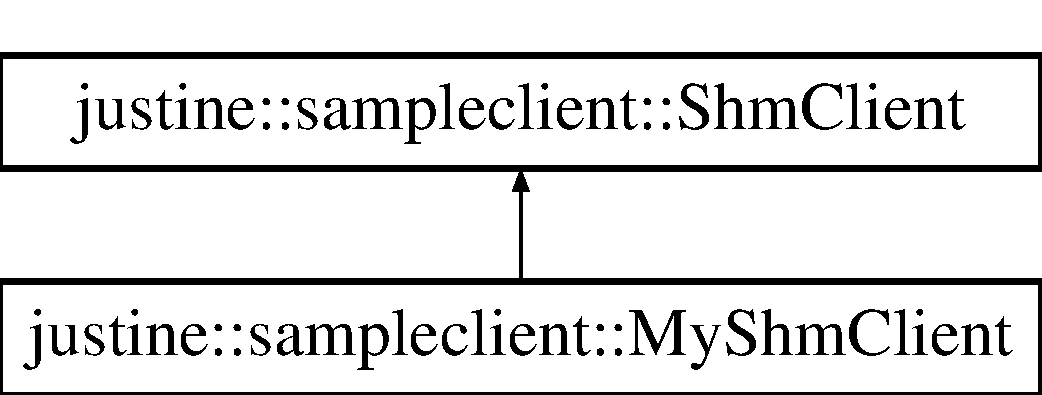
\includegraphics[height=2.000000cm]{classjustine_1_1sampleclient_1_1MyShmClient}
\end{center}
\end{figure}
\subsection*{Public Member Functions}
\begin{DoxyCompactItemize}
\item 
\hyperlink{classjustine_1_1sampleclient_1_1MyShmClient_a7e7a693ff4d4eb7eda923413aa1b26c2}{My\-Shm\-Client} (const char $\ast$shm\-\_\-segment, std\-::string teamname)
\begin{DoxyCompactList}\small\item\em This constructor creates the B\-G\-L graph from the map graph. \end{DoxyCompactList}\item 
\hypertarget{classjustine_1_1sampleclient_1_1MyShmClient_abab9d1fcda42de37996cd169aff36e03}{\hyperlink{classjustine_1_1sampleclient_1_1MyShmClient_abab9d1fcda42de37996cd169aff36e03}{$\sim$\-My\-Shm\-Client} ()}\label{classjustine_1_1sampleclient_1_1MyShmClient_abab9d1fcda42de37996cd169aff36e03}

\begin{DoxyCompactList}\small\item\em Dtor. \end{DoxyCompactList}\item 
void \hyperlink{classjustine_1_1sampleclient_1_1MyShmClient_aa5cb338eade5f427f4a82b28cff4ca14}{start} (boost\-::asio\-::io\-\_\-service \&io\-\_\-service, const char $\ast$port)
\begin{DoxyCompactList}\small\item\em This function starts the client. \end{DoxyCompactList}\item 
\hypertarget{classjustine_1_1sampleclient_1_1MyShmClient_a14dc5382a149b98327d71e8fb6548bd1}{void {\bfseries start10} (boost\-::asio\-::io\-\_\-service \&io\-\_\-service, const char $\ast$port)}\label{classjustine_1_1sampleclient_1_1MyShmClient_a14dc5382a149b98327d71e8fb6548bd1}

\item 
int \hyperlink{classjustine_1_1sampleclient_1_1MyShmClient_a660a0217e0413f4e5f6c1bfc2be80834}{num\-\_\-vertices} (int \&sum\-\_\-edges)
\begin{DoxyCompactList}\small\item\em This function counts the number of vertices and number of edges in the map graph. \end{DoxyCompactList}\item 
void \hyperlink{classjustine_1_1sampleclient_1_1MyShmClient_ad92c09f0803a99cd3c523063b4339420}{print\-\_\-edges} (unsigned more)
\begin{DoxyCompactList}\small\item\em This function prints the edges of the map graph. \end{DoxyCompactList}\item 
void \hyperlink{classjustine_1_1sampleclient_1_1MyShmClient_ad715aff6797601f785e74bc83906e366}{print\-\_\-vertices} (unsigned more)
\begin{DoxyCompactList}\small\item\em This function prints the vertices of the map graph. \end{DoxyCompactList}\item 
Node\-Ref\-Graph $\ast$ \hyperlink{classjustine_1_1sampleclient_1_1MyShmClient_a3f164bc7db036f35477f82f5d837ac17}{bgl\-\_\-graph} (void)
\begin{DoxyCompactList}\small\item\em This function create the B\-G\-L graph. \end{DoxyCompactList}\item 
std\-::vector\\*
$<$ osmium\-::unsigned\-\_\-object\-\_\-id\-\_\-type $>$ \hyperlink{classjustine_1_1sampleclient_1_1MyShmClient_a84e9fce2ea4e84c0d54f930cbfb3b889}{has\-Dijkstra\-Path} (osmium\-::unsigned\-\_\-object\-\_\-id\-\_\-type from, osmium\-::unsigned\-\_\-object\-\_\-id\-\_\-type to)
\begin{DoxyCompactList}\small\item\em This function solves the shortest path problem using Dijkstra algorithm. \end{DoxyCompactList}\item 
std\-::vector\\*
$<$ osmium\-::unsigned\-\_\-object\-\_\-id\-\_\-type $>$ \hyperlink{classjustine_1_1sampleclient_1_1MyShmClient_a09309cb534eb586e5a9a1954e3e4c7d9}{has\-Bellman\-Ford\-Path} (osmium\-::unsigned\-\_\-object\-\_\-id\-\_\-type from, osmium\-::unsigned\-\_\-object\-\_\-id\-\_\-type to)
\begin{DoxyCompactList}\small\item\em This function solves the shortest path problem using Bellman-\/\-Ford algorithm. \end{DoxyCompactList}\end{DoxyCompactItemize}
\subsection*{Protected Attributes}
\begin{DoxyCompactItemize}
\item 
\hypertarget{classjustine_1_1sampleclient_1_1MyShmClient_a92bf3aebaf3fa90424a5bec8b3c34e9a}{Node\-Ref\-Graph $\ast$ {\bfseries nr\-\_\-graph}}\label{classjustine_1_1sampleclient_1_1MyShmClient_a92bf3aebaf3fa90424a5bec8b3c34e9a}

\item 
\hypertarget{classjustine_1_1sampleclient_1_1MyShmClient_ab0411a2dbad884643f1112183152875a}{std\-::string {\bfseries m\-\_\-teamname}}\label{classjustine_1_1sampleclient_1_1MyShmClient_ab0411a2dbad884643f1112183152875a}

\end{DoxyCompactItemize}


\subsection{Detailed Description}
A sample class used for testing the routing algorithms. 

This sample class shows how client agents can create B\-G\-L graph from data can be found in the shared memory.

\begin{DoxyAuthor}{Author}
Norbert Bátfai 
\end{DoxyAuthor}
\begin{DoxyDate}{Date}
Dec. 7, 2014 
\end{DoxyDate}


Definition at line 105 of file myshmclient.\-hpp.



\subsection{Constructor \& Destructor Documentation}
\hypertarget{classjustine_1_1sampleclient_1_1MyShmClient_a7e7a693ff4d4eb7eda923413aa1b26c2}{\index{justine\-::sampleclient\-::\-My\-Shm\-Client@{justine\-::sampleclient\-::\-My\-Shm\-Client}!My\-Shm\-Client@{My\-Shm\-Client}}
\index{My\-Shm\-Client@{My\-Shm\-Client}!justine::sampleclient::MyShmClient@{justine\-::sampleclient\-::\-My\-Shm\-Client}}
\subsubsection[{My\-Shm\-Client}]{\setlength{\rightskip}{0pt plus 5cm}justine\-::sampleclient\-::\-My\-Shm\-Client\-::\-My\-Shm\-Client (
\begin{DoxyParamCaption}
\item[{const char $\ast$}]{shm\-\_\-segment, }
\item[{std\-::string}]{teamname}
\end{DoxyParamCaption}
)\hspace{0.3cm}{\ttfamily [inline]}}}\label{classjustine_1_1sampleclient_1_1MyShmClient_a7e7a693ff4d4eb7eda923413aa1b26c2}


This constructor creates the B\-G\-L graph from the map graph. 


\begin{DoxyParams}{Parameters}
{\em shm\-\_\-segment} & the shared memory object name\\
\hline
\end{DoxyParams}
This constructor creates the B\-G\-L graph from the map graph that is placed in the shared memory segment. 

Definition at line 116 of file myshmclient.\-hpp.



\subsection{Member Function Documentation}
\hypertarget{classjustine_1_1sampleclient_1_1MyShmClient_a3f164bc7db036f35477f82f5d837ac17}{\index{justine\-::sampleclient\-::\-My\-Shm\-Client@{justine\-::sampleclient\-::\-My\-Shm\-Client}!bgl\-\_\-graph@{bgl\-\_\-graph}}
\index{bgl\-\_\-graph@{bgl\-\_\-graph}!justine::sampleclient::MyShmClient@{justine\-::sampleclient\-::\-My\-Shm\-Client}}
\subsubsection[{bgl\-\_\-graph}]{\setlength{\rightskip}{0pt plus 5cm}Node\-Ref\-Graph$\ast$ justine\-::sampleclient\-::\-My\-Shm\-Client\-::bgl\-\_\-graph (
\begin{DoxyParamCaption}
\item[{void}]{}
\end{DoxyParamCaption}
)\hspace{0.3cm}{\ttfamily [inline]}}}\label{classjustine_1_1sampleclient_1_1MyShmClient_a3f164bc7db036f35477f82f5d837ac17}


This function create the B\-G\-L graph. 

\begin{DoxyReturn}{Returns}
he pointer of the created B\-G\-L graph. 
\end{DoxyReturn}


Definition at line 249 of file myshmclient.\-hpp.

\hypertarget{classjustine_1_1sampleclient_1_1MyShmClient_a09309cb534eb586e5a9a1954e3e4c7d9}{\index{justine\-::sampleclient\-::\-My\-Shm\-Client@{justine\-::sampleclient\-::\-My\-Shm\-Client}!has\-Bellman\-Ford\-Path@{has\-Bellman\-Ford\-Path}}
\index{has\-Bellman\-Ford\-Path@{has\-Bellman\-Ford\-Path}!justine::sampleclient::MyShmClient@{justine\-::sampleclient\-::\-My\-Shm\-Client}}
\subsubsection[{has\-Bellman\-Ford\-Path}]{\setlength{\rightskip}{0pt plus 5cm}std\-::vector$<$osmium\-::unsigned\-\_\-object\-\_\-id\-\_\-type$>$ justine\-::sampleclient\-::\-My\-Shm\-Client\-::has\-Bellman\-Ford\-Path (
\begin{DoxyParamCaption}
\item[{osmium\-::unsigned\-\_\-object\-\_\-id\-\_\-type}]{from, }
\item[{osmium\-::unsigned\-\_\-object\-\_\-id\-\_\-type}]{to}
\end{DoxyParamCaption}
)\hspace{0.3cm}{\ttfamily [inline]}}}\label{classjustine_1_1sampleclient_1_1MyShmClient_a09309cb534eb586e5a9a1954e3e4c7d9}


This function solves the shortest path problem using Bellman-\/\-Ford algorithm. 


\begin{DoxyParams}{Parameters}
{\em source} & the source node \\
\hline
{\em target} & the target node \\
\hline
\end{DoxyParams}
\begin{DoxyReturn}{Returns}
the shortest path between nodes source and target
\end{DoxyReturn}
This function determines the shortest path from the source node to the target node. 

Definition at line 400 of file myshmclient.\-hpp.

\hypertarget{classjustine_1_1sampleclient_1_1MyShmClient_a84e9fce2ea4e84c0d54f930cbfb3b889}{\index{justine\-::sampleclient\-::\-My\-Shm\-Client@{justine\-::sampleclient\-::\-My\-Shm\-Client}!has\-Dijkstra\-Path@{has\-Dijkstra\-Path}}
\index{has\-Dijkstra\-Path@{has\-Dijkstra\-Path}!justine::sampleclient::MyShmClient@{justine\-::sampleclient\-::\-My\-Shm\-Client}}
\subsubsection[{has\-Dijkstra\-Path}]{\setlength{\rightskip}{0pt plus 5cm}std\-::vector$<$osmium\-::unsigned\-\_\-object\-\_\-id\-\_\-type$>$ justine\-::sampleclient\-::\-My\-Shm\-Client\-::has\-Dijkstra\-Path (
\begin{DoxyParamCaption}
\item[{osmium\-::unsigned\-\_\-object\-\_\-id\-\_\-type}]{from, }
\item[{osmium\-::unsigned\-\_\-object\-\_\-id\-\_\-type}]{to}
\end{DoxyParamCaption}
)\hspace{0.3cm}{\ttfamily [inline]}}}\label{classjustine_1_1sampleclient_1_1MyShmClient_a84e9fce2ea4e84c0d54f930cbfb3b889}


This function solves the shortest path problem using Dijkstra algorithm. 


\begin{DoxyParams}{Parameters}
{\em source} & the source node \\
\hline
{\em target} & the target node \\
\hline
\end{DoxyParams}
\begin{DoxyReturn}{Returns}
the shortest path between nodes source and target
\end{DoxyReturn}
This function determines the shortest path from the source node to the target node. 

Definition at line 329 of file myshmclient.\-hpp.

\hypertarget{classjustine_1_1sampleclient_1_1MyShmClient_a660a0217e0413f4e5f6c1bfc2be80834}{\index{justine\-::sampleclient\-::\-My\-Shm\-Client@{justine\-::sampleclient\-::\-My\-Shm\-Client}!num\-\_\-vertices@{num\-\_\-vertices}}
\index{num\-\_\-vertices@{num\-\_\-vertices}!justine::sampleclient::MyShmClient@{justine\-::sampleclient\-::\-My\-Shm\-Client}}
\subsubsection[{num\-\_\-vertices}]{\setlength{\rightskip}{0pt plus 5cm}int justine\-::sampleclient\-::\-My\-Shm\-Client\-::num\-\_\-vertices (
\begin{DoxyParamCaption}
\item[{int \&}]{sum\-\_\-edges}
\end{DoxyParamCaption}
)\hspace{0.3cm}{\ttfamily [inline]}}}\label{classjustine_1_1sampleclient_1_1MyShmClient_a660a0217e0413f4e5f6c1bfc2be80834}


This function counts the number of vertices and number of edges in the map graph. 


\begin{DoxyParams}[1]{Parameters}
\mbox{\tt out}  & {\em sum\-\_\-edges} & the number of edges \\
\hline
\end{DoxyParams}
\begin{DoxyReturn}{Returns}
the number of vertices
\end{DoxyReturn}
This function counts the number of vertices and number of edges in the map graph that is placed in the shared memory segment. 

Definition at line 162 of file myshmclient.\-hpp.

\hypertarget{classjustine_1_1sampleclient_1_1MyShmClient_ad92c09f0803a99cd3c523063b4339420}{\index{justine\-::sampleclient\-::\-My\-Shm\-Client@{justine\-::sampleclient\-::\-My\-Shm\-Client}!print\-\_\-edges@{print\-\_\-edges}}
\index{print\-\_\-edges@{print\-\_\-edges}!justine::sampleclient::MyShmClient@{justine\-::sampleclient\-::\-My\-Shm\-Client}}
\subsubsection[{print\-\_\-edges}]{\setlength{\rightskip}{0pt plus 5cm}void justine\-::sampleclient\-::\-My\-Shm\-Client\-::print\-\_\-edges (
\begin{DoxyParamCaption}
\item[{unsigned}]{more}
\end{DoxyParamCaption}
)\hspace{0.3cm}{\ttfamily [inline]}}}\label{classjustine_1_1sampleclient_1_1MyShmClient_ad92c09f0803a99cd3c523063b4339420}


This function prints the edges of the map graph. 


\begin{DoxyParams}{Parameters}
{\em more} & the maximum number of printed items \\
\hline
\end{DoxyParams}


Definition at line 189 of file myshmclient.\-hpp.

\hypertarget{classjustine_1_1sampleclient_1_1MyShmClient_ad715aff6797601f785e74bc83906e366}{\index{justine\-::sampleclient\-::\-My\-Shm\-Client@{justine\-::sampleclient\-::\-My\-Shm\-Client}!print\-\_\-vertices@{print\-\_\-vertices}}
\index{print\-\_\-vertices@{print\-\_\-vertices}!justine::sampleclient::MyShmClient@{justine\-::sampleclient\-::\-My\-Shm\-Client}}
\subsubsection[{print\-\_\-vertices}]{\setlength{\rightskip}{0pt plus 5cm}void justine\-::sampleclient\-::\-My\-Shm\-Client\-::print\-\_\-vertices (
\begin{DoxyParamCaption}
\item[{unsigned}]{more}
\end{DoxyParamCaption}
)\hspace{0.3cm}{\ttfamily [inline]}}}\label{classjustine_1_1sampleclient_1_1MyShmClient_ad715aff6797601f785e74bc83906e366}


This function prints the vertices of the map graph. 


\begin{DoxyParams}{Parameters}
{\em more} & the maximum number of printed items \\
\hline
\end{DoxyParams}


Definition at line 214 of file myshmclient.\-hpp.

\hypertarget{classjustine_1_1sampleclient_1_1MyShmClient_aa5cb338eade5f427f4a82b28cff4ca14}{\index{justine\-::sampleclient\-::\-My\-Shm\-Client@{justine\-::sampleclient\-::\-My\-Shm\-Client}!start@{start}}
\index{start@{start}!justine::sampleclient::MyShmClient@{justine\-::sampleclient\-::\-My\-Shm\-Client}}
\subsubsection[{start}]{\setlength{\rightskip}{0pt plus 5cm}void justine\-::sampleclient\-::\-My\-Shm\-Client\-::start (
\begin{DoxyParamCaption}
\item[{boost\-::asio\-::io\-\_\-service \&}]{io\-\_\-service, }
\item[{const char $\ast$}]{port}
\end{DoxyParamCaption}
)}}\label{classjustine_1_1sampleclient_1_1MyShmClient_aa5cb338eade5f427f4a82b28cff4ca14}


This function starts the client. 


\begin{DoxyParams}{Parameters}
{\em io\-\_\-service} & \\
\hline
{\em port} & the T\-C\-P port of the traffic server\\
\hline
\end{DoxyParams}
This method does the following\-: retrieves a value from shared memory, then establishes a connection with the traffic server, finally sends some client commands. 

Definition at line 265 of file myshmclient.\-cpp.



The documentation for this class was generated from the following files\-:\begin{DoxyCompactItemize}
\item 
src/\hyperlink{myshmclient_8hpp}{myshmclient.\-hpp}\item 
src/\hyperlink{myshmclient_8cpp}{myshmclient.\-cpp}\end{DoxyCompactItemize}

\hypertarget{classjustine_1_1robocar_1_1OSMReader}{\section{justine\-:\-:robocar\-:\-:O\-S\-M\-Reader Class Reference}
\label{classjustine_1_1robocar_1_1OSMReader}\index{justine\-::robocar\-::\-O\-S\-M\-Reader@{justine\-::robocar\-::\-O\-S\-M\-Reader}}
}
Inheritance diagram for justine\-:\-:robocar\-:\-:O\-S\-M\-Reader\-:\begin{figure}[H]
\begin{center}
\leavevmode
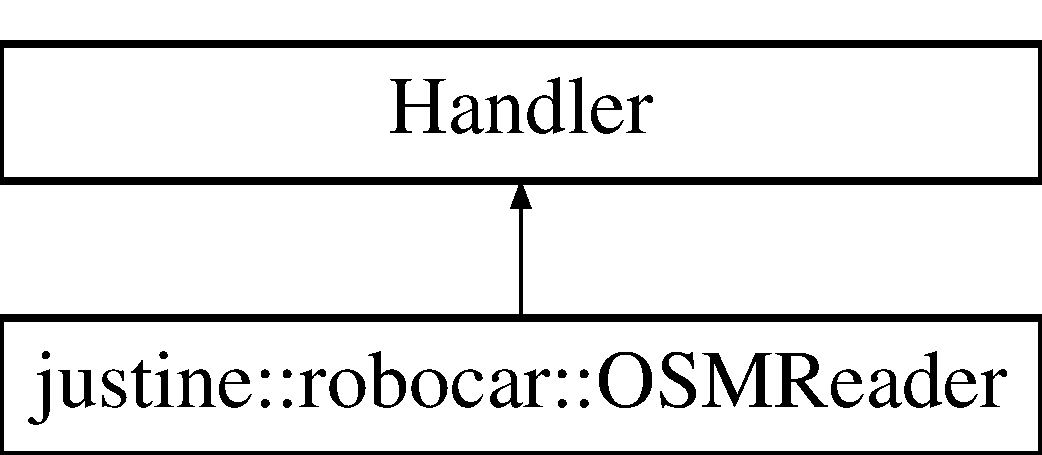
\includegraphics[height=2.000000cm]{classjustine_1_1robocar_1_1OSMReader}
\end{center}
\end{figure}
\subsection*{Public Member Functions}
\begin{DoxyCompactItemize}
\item 
\hypertarget{classjustine_1_1robocar_1_1OSMReader_aec040325b35f2d2d7da1f4fe374fa123}{{\bfseries O\-S\-M\-Reader} (const char $\ast$osm\-\_\-file, Adjacency\-List \&alist, Adjacency\-List \&palist, Waynode\-Locations \&waynode\-\_\-locations, Way\-Nodes\-Map \&bus\-Way\-Nodes\-Map, Way2\-Nodes \&way2nodes)}\label{classjustine_1_1robocar_1_1OSMReader_aec040325b35f2d2d7da1f4fe374fa123}

\item 
\hypertarget{classjustine_1_1robocar_1_1OSMReader_a299192923af868d17a9e789f9a393fc9}{std\-::size\-\_\-t {\bfseries get\-\_\-estimated\-\_\-memory} () const }\label{classjustine_1_1robocar_1_1OSMReader_a299192923af868d17a9e789f9a393fc9}

\item 
\hypertarget{classjustine_1_1robocar_1_1OSMReader_afbb52b817781b4f700db6946ebdffa4d}{bool {\bfseries edge} (osmium\-::unsigned\-\_\-object\-\_\-id\-\_\-type v1, osmium\-::unsigned\-\_\-object\-\_\-id\-\_\-type v2)}\label{classjustine_1_1robocar_1_1OSMReader_afbb52b817781b4f700db6946ebdffa4d}

\item 
\hypertarget{classjustine_1_1robocar_1_1OSMReader_a09b77083902c6b8e65783ff44f1f16b5}{void {\bfseries node} (osmium\-::\-Node \&node)}\label{classjustine_1_1robocar_1_1OSMReader_a09b77083902c6b8e65783ff44f1f16b5}

\item 
\hypertarget{classjustine_1_1robocar_1_1OSMReader_a370575ff1c26042b43a69d8a80a4d4a1}{void {\bfseries way} (osmium\-::\-Way \&way)}\label{classjustine_1_1robocar_1_1OSMReader_a370575ff1c26042b43a69d8a80a4d4a1}

\item 
\hypertarget{classjustine_1_1robocar_1_1OSMReader_a7c9c0aae3bc3bcfc9d83ddbc1c13ef6c}{void {\bfseries relation} (osmium\-::\-Relation \&rel)}\label{classjustine_1_1robocar_1_1OSMReader_a7c9c0aae3bc3bcfc9d83ddbc1c13ef6c}

\end{DoxyCompactItemize}
\subsection*{Public Attributes}
\begin{DoxyCompactItemize}
\item 
\hypertarget{classjustine_1_1robocar_1_1OSMReader_a634019bf205c563f37a534f8a0875a63}{int {\bfseries onewayc} \{0\}}\label{classjustine_1_1robocar_1_1OSMReader_a634019bf205c563f37a534f8a0875a63}

\item 
\hypertarget{classjustine_1_1robocar_1_1OSMReader_a1bf3e852c9e168b69c6e06492883d6b6}{int {\bfseries onewayf} \{false\}}\label{classjustine_1_1robocar_1_1OSMReader_a1bf3e852c9e168b69c6e06492883d6b6}

\end{DoxyCompactItemize}
\subsection*{Protected Attributes}
\begin{DoxyCompactItemize}
\item 
\hypertarget{classjustine_1_1robocar_1_1OSMReader_a5ee6d6b2ff2387d2910c1ff7a8b096c2}{Vertices {\bfseries vert}}\label{classjustine_1_1robocar_1_1OSMReader_a5ee6d6b2ff2387d2910c1ff7a8b096c2}

\item 
\hypertarget{classjustine_1_1robocar_1_1OSMReader_a4861c9c3fa4d4efd3c4257bc3f413f52}{int {\bfseries n\-O\-S\-M\-\_\-nodes} \{0\}}\label{classjustine_1_1robocar_1_1OSMReader_a4861c9c3fa4d4efd3c4257bc3f413f52}

\item 
\hypertarget{classjustine_1_1robocar_1_1OSMReader_ad6b041b730a1b8e19463616d45c656d8}{int {\bfseries n\-O\-S\-M\-\_\-ways} \{0\}}\label{classjustine_1_1robocar_1_1OSMReader_ad6b041b730a1b8e19463616d45c656d8}

\item 
\hypertarget{classjustine_1_1robocar_1_1OSMReader_ac1fff059cfdd893ef4ef75538ee65852}{int {\bfseries n\-O\-S\-M\-\_\-relations} \{0\}}\label{classjustine_1_1robocar_1_1OSMReader_ac1fff059cfdd893ef4ef75538ee65852}

\item 
\hypertarget{classjustine_1_1robocar_1_1OSMReader_a7d4de71f87767cb4605a94cd02abe3c8}{int {\bfseries sum\-\_\-unique\-\_\-highhway\-\_\-nodes} \{0\}}\label{classjustine_1_1robocar_1_1OSMReader_a7d4de71f87767cb4605a94cd02abe3c8}

\item 
\hypertarget{classjustine_1_1robocar_1_1OSMReader_ae4cffb00fde3690b29dd014be6b89b82}{int {\bfseries sum\-\_\-highhway\-\_\-nodes} \{0\}}\label{classjustine_1_1robocar_1_1OSMReader_ae4cffb00fde3690b29dd014be6b89b82}

\item 
\hypertarget{classjustine_1_1robocar_1_1OSMReader_a719895a0386e0df8ce8d9d756b22a5f1}{int {\bfseries sum\-\_\-highhway\-\_\-length} \{0\}}\label{classjustine_1_1robocar_1_1OSMReader_a719895a0386e0df8ce8d9d756b22a5f1}

\item 
\hypertarget{classjustine_1_1robocar_1_1OSMReader_aac15fee813882d75772a2cc5fa150117}{int {\bfseries edge\-\_\-multiplicity} = 0}\label{classjustine_1_1robocar_1_1OSMReader_aac15fee813882d75772a2cc5fa150117}

\item 
\hypertarget{classjustine_1_1robocar_1_1OSMReader_ac9c3c5b225616c42affc70ad7c166cbf}{int {\bfseries nbuses} \{0\}}\label{classjustine_1_1robocar_1_1OSMReader_ac9c3c5b225616c42affc70ad7c166cbf}

\item 
\hypertarget{classjustine_1_1robocar_1_1OSMReader_ae18da4de7dd3f160bfee6c9617d8dbd2}{double {\bfseries max\-\_\-edge\-\_\-length} \{0.\-0\}}\label{classjustine_1_1robocar_1_1OSMReader_ae18da4de7dd3f160bfee6c9617d8dbd2}

\item 
\hypertarget{classjustine_1_1robocar_1_1OSMReader_a11ccc11ef3622245ab62c71740afa5e2}{double {\bfseries mean\-\_\-edge\-\_\-length} \{0.\-0\}}\label{classjustine_1_1robocar_1_1OSMReader_a11ccc11ef3622245ab62c71740afa5e2}

\item 
\hypertarget{classjustine_1_1robocar_1_1OSMReader_acc08941b57ee58d87dcb9351b936dcfa}{int {\bfseries cedges} \{0\}}\label{classjustine_1_1robocar_1_1OSMReader_acc08941b57ee58d87dcb9351b936dcfa}

\item 
\hypertarget{classjustine_1_1robocar_1_1OSMReader_acf4fd66c1058ee90ad34806e571bb1c1}{O\-S\-M\-Locations {\bfseries locations}}\label{classjustine_1_1robocar_1_1OSMReader_acf4fd66c1058ee90ad34806e571bb1c1}

\end{DoxyCompactItemize}


\subsection{Detailed Description}


Definition at line 72 of file osmreader.\-hpp.



The documentation for this class was generated from the following file\-:\begin{DoxyCompactItemize}
\item 
src/\hyperlink{osmreader_8hpp}{osmreader.\-hpp}\end{DoxyCompactItemize}

\hypertarget{classjustine_1_1robocar_1_1SharedData}{\section{justine\-:\-:robocar\-:\-:Shared\-Data Class Reference}
\label{classjustine_1_1robocar_1_1SharedData}\index{justine\-::robocar\-::\-Shared\-Data@{justine\-::robocar\-::\-Shared\-Data}}
}
\subsection*{Public Member Functions}
\begin{DoxyCompactItemize}
\item 
\hypertarget{classjustine_1_1robocar_1_1SharedData_a87c2651f40582aedd62f9d9c3b6c8459}{{\bfseries Shared\-Data} (const void\-\_\-allocator \&void\-\_\-alloc)}\label{classjustine_1_1robocar_1_1SharedData_a87c2651f40582aedd62f9d9c3b6c8459}

\end{DoxyCompactItemize}
\subsection*{Public Attributes}
\begin{DoxyCompactItemize}
\item 
\hypertarget{classjustine_1_1robocar_1_1SharedData_a3630c63f80d3b75d91fe59829e001e57}{uint\-\_\-vector {\bfseries m\-\_\-alist}}\label{classjustine_1_1robocar_1_1SharedData_a3630c63f80d3b75d91fe59829e001e57}

\item 
\hypertarget{classjustine_1_1robocar_1_1SharedData_a778d32b1551d9fbd6c8c1a6aa3a8cf1d}{uint\-\_\-vector {\bfseries m\-\_\-salist}}\label{classjustine_1_1robocar_1_1SharedData_a778d32b1551d9fbd6c8c1a6aa3a8cf1d}

\item 
\hypertarget{classjustine_1_1robocar_1_1SharedData_a1a38db5cffcb433f5635f1953b8774f3}{uint\-\_\-vector {\bfseries m\-\_\-palist}}\label{classjustine_1_1robocar_1_1SharedData_a1a38db5cffcb433f5635f1953b8774f3}

\item 
\hypertarget{classjustine_1_1robocar_1_1SharedData_a25ee774ed2ae16e69d16daafedb94fa4}{int {\bfseries lon}}\label{classjustine_1_1robocar_1_1SharedData_a25ee774ed2ae16e69d16daafedb94fa4}

\item 
\hypertarget{classjustine_1_1robocar_1_1SharedData_a211fcd1fefd4788728a0f322ab53609e}{int {\bfseries lat}}\label{classjustine_1_1robocar_1_1SharedData_a211fcd1fefd4788728a0f322ab53609e}

\end{DoxyCompactItemize}


\subsection{Detailed Description}


Definition at line 62 of file smartcity.\-hpp.



The documentation for this class was generated from the following file\-:\begin{DoxyCompactItemize}
\item 
src/\hyperlink{smartcity_8hpp}{smartcity.\-hpp}\end{DoxyCompactItemize}

\hypertarget{classjustine_1_1sampleclient_1_1ShmClient}{\section{justine\-:\-:sampleclient\-:\-:Shm\-Client Class Reference}
\label{classjustine_1_1sampleclient_1_1ShmClient}\index{justine\-::sampleclient\-::\-Shm\-Client@{justine\-::sampleclient\-::\-Shm\-Client}}
}


A sample class used for testing I\-P\-C mechanisms (S\-H\-M and sockets) which are used by the city emulator.  




{\ttfamily \#include $<$shmclient.\-hpp$>$}

Inheritance diagram for justine\-:\-:sampleclient\-:\-:Shm\-Client\-:\begin{figure}[H]
\begin{center}
\leavevmode
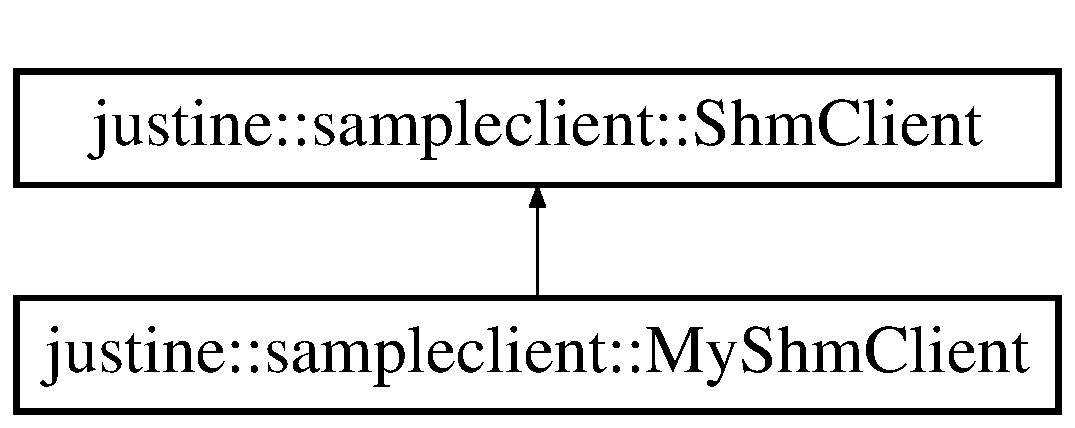
\includegraphics[height=2.000000cm]{classjustine_1_1sampleclient_1_1ShmClient}
\end{center}
\end{figure}
\subsection*{Public Member Functions}
\begin{DoxyCompactItemize}
\item 
\hyperlink{classjustine_1_1sampleclient_1_1ShmClient_a7b12c596ecc920351b2c12bbfeeee7e2}{Shm\-Client} (const char $\ast$shm\-\_\-segment)
\begin{DoxyCompactList}\small\item\em This constructor initializes the shared memory segment. \end{DoxyCompactList}\item 
void \hyperlink{classjustine_1_1sampleclient_1_1ShmClient_a7a88330a12e2a0cbfbfabae4891b3021}{start} (boost\-::asio\-::io\-\_\-service \&io\-\_\-service, const char $\ast$port)
\begin{DoxyCompactList}\small\item\em This function starts the client. \end{DoxyCompactList}\item 
virtual \\*
osmium\-::unsigned\-\_\-object\-\_\-id\-\_\-type \hyperlink{classjustine_1_1sampleclient_1_1ShmClient_aa4c2f16ec6d72aec8070c683d5b789be}{get\-\_\-random\-\_\-node} (void)
\begin{DoxyCompactList}\small\item\em This function returns a randomly chosen node from the map. \end{DoxyCompactList}\item 
size\-\_\-t \hyperlink{classjustine_1_1sampleclient_1_1ShmClient_a959359ddb659c32f1f65253e2359ea4f}{num\-\_\-edges} (osmium\-::unsigned\-\_\-object\-\_\-id\-\_\-type from) const 
\begin{DoxyCompactList}\small\item\em Returns the number of out edges of a given vertex. \end{DoxyCompactList}\item 
osmium\-::unsigned\-\_\-object\-\_\-id\-\_\-type \hyperlink{classjustine_1_1sampleclient_1_1ShmClient_a35581aba18f1c16b440dd50e84dc7715}{alist} (osmium\-::unsigned\-\_\-object\-\_\-id\-\_\-type from, int to) const 
\begin{DoxyCompactList}\small\item\em Returns the i-\/th neighbor of the actual vertex. \end{DoxyCompactList}\item 
\hypertarget{classjustine_1_1sampleclient_1_1ShmClient_a652b7137db56feb4de93ffce057ffbf9}{int {\bfseries alist\-\_\-inv} (osmium\-::unsigned\-\_\-object\-\_\-id\-\_\-type from, osmium\-::unsigned\-\_\-object\-\_\-id\-\_\-type to) const }\label{classjustine_1_1sampleclient_1_1ShmClient_a652b7137db56feb4de93ffce057ffbf9}

\item 
\hypertarget{classjustine_1_1sampleclient_1_1ShmClient_aaa91265eefc33bb73d55989e8074b3d8}{osmium\-::unsigned\-\_\-object\-\_\-id\-\_\-type {\bfseries salist} (osmium\-::unsigned\-\_\-object\-\_\-id\-\_\-type from, int to) const }\label{classjustine_1_1sampleclient_1_1ShmClient_aaa91265eefc33bb73d55989e8074b3d8}

\item 
\hypertarget{classjustine_1_1sampleclient_1_1ShmClient_a5b2928e2dd538c5712c9302e940770f8}{void {\bfseries set\-\_\-salist} (osmium\-::unsigned\-\_\-object\-\_\-id\-\_\-type from, int to, osmium\-::unsigned\-\_\-object\-\_\-id\-\_\-type value)}\label{classjustine_1_1sampleclient_1_1ShmClient_a5b2928e2dd538c5712c9302e940770f8}

\item 
\hypertarget{classjustine_1_1sampleclient_1_1ShmClient_a88e09b87f6f91f0961821731d578397c}{osmium\-::unsigned\-\_\-object\-\_\-id\-\_\-type {\bfseries palist} (osmium\-::unsigned\-\_\-object\-\_\-id\-\_\-type from, int to) const }\label{classjustine_1_1sampleclient_1_1ShmClient_a88e09b87f6f91f0961821731d578397c}

\item 
\hypertarget{classjustine_1_1sampleclient_1_1ShmClient_a7d6d4258adcfc4753b025d3a10239bb3}{bool {\bfseries has\-Node} (osmium\-::unsigned\-\_\-object\-\_\-id\-\_\-type node)}\label{classjustine_1_1sampleclient_1_1ShmClient_a7d6d4258adcfc4753b025d3a10239bb3}

\item 
\hypertarget{classjustine_1_1sampleclient_1_1ShmClient_a81901cf4e8b7ea0ed416b7a0773d0893}{double {\bfseries dst} (osmium\-::unsigned\-\_\-object\-\_\-id\-\_\-type n1, osmium\-::unsigned\-\_\-object\-\_\-id\-\_\-type n2) const }\label{classjustine_1_1sampleclient_1_1ShmClient_a81901cf4e8b7ea0ed416b7a0773d0893}

\item 
\hypertarget{classjustine_1_1sampleclient_1_1ShmClient_ae1a1cd61d7de906362bb95a38e65cd24}{double {\bfseries dst} (double lon1, double lat1, double lon2, double lat2) const }\label{classjustine_1_1sampleclient_1_1ShmClient_ae1a1cd61d7de906362bb95a38e65cd24}

\item 
\hypertarget{classjustine_1_1sampleclient_1_1ShmClient_a4d5965a9626d92ded45dbb01c0e4ac28}{void {\bfseries to\-G\-P\-S} (osmium\-::unsigned\-\_\-object\-\_\-id\-\_\-type from, double $\ast$lo, double $\ast$la) const }\label{classjustine_1_1sampleclient_1_1ShmClient_a4d5965a9626d92ded45dbb01c0e4ac28}

\item 
\hypertarget{classjustine_1_1sampleclient_1_1ShmClient_a632e85bed10638ec836db5132fc50a54}{void {\bfseries to\-G\-P\-S} (osmium\-::unsigned\-\_\-object\-\_\-id\-\_\-type from, osmium\-::unsigned\-\_\-object\-\_\-id\-\_\-type to, osmium\-::unsigned\-\_\-object\-\_\-id\-\_\-type step, double $\ast$lo, double $\ast$la) const }\label{classjustine_1_1sampleclient_1_1ShmClient_a632e85bed10638ec836db5132fc50a54}

\end{DoxyCompactItemize}
\subsection*{Protected Attributes}
\begin{DoxyCompactItemize}
\item 
\hypertarget{classjustine_1_1sampleclient_1_1ShmClient_a7ccabc4f33d08ebbcd0099033d18ce21}{boost\-::interprocess\-::offset\-\_\-ptr\\*
$<$ justine\-::robocar\-::shm\-\_\-map\-\_\-\-Type $>$ \hyperlink{classjustine_1_1sampleclient_1_1ShmClient_a7ccabc4f33d08ebbcd0099033d18ce21}{shm\-\_\-map}}\label{classjustine_1_1sampleclient_1_1ShmClient_a7ccabc4f33d08ebbcd0099033d18ce21}

\begin{DoxyCompactList}\small\item\em The O\-S\-M map data stored in a shared memory segment. \end{DoxyCompactList}\end{DoxyCompactItemize}


\subsection{Detailed Description}
A sample class used for testing I\-P\-C mechanisms (S\-H\-M and sockets) which are used by the city emulator. 

This sample class shows how client agents can connect and communicate with traffic emulator using shared memory.

\begin{DoxyAuthor}{Author}
Norbert Bátfai 
\end{DoxyAuthor}
\begin{DoxyDate}{Date}
Dec. 7, 2014 
\end{DoxyDate}


Definition at line 66 of file shmclient.\-hpp.



\subsection{Constructor \& Destructor Documentation}
\hypertarget{classjustine_1_1sampleclient_1_1ShmClient_a7b12c596ecc920351b2c12bbfeeee7e2}{\index{justine\-::sampleclient\-::\-Shm\-Client@{justine\-::sampleclient\-::\-Shm\-Client}!Shm\-Client@{Shm\-Client}}
\index{Shm\-Client@{Shm\-Client}!justine::sampleclient::ShmClient@{justine\-::sampleclient\-::\-Shm\-Client}}
\subsubsection[{Shm\-Client}]{\setlength{\rightskip}{0pt plus 5cm}justine\-::sampleclient\-::\-Shm\-Client\-::\-Shm\-Client (
\begin{DoxyParamCaption}
\item[{const char $\ast$}]{shm\-\_\-segment}
\end{DoxyParamCaption}
)\hspace{0.3cm}{\ttfamily [inline]}}}\label{classjustine_1_1sampleclient_1_1ShmClient_a7b12c596ecc920351b2c12bbfeeee7e2}


This constructor initializes the shared memory segment. 


\begin{DoxyParams}{Parameters}
{\em shm\-\_\-segment} & the shared memory object name\\
\hline
\end{DoxyParams}
This constructor attaches the shared memory segment identified by the param shm\-\_\-segment. 

Definition at line 76 of file shmclient.\-hpp.



\subsection{Member Function Documentation}
\hypertarget{classjustine_1_1sampleclient_1_1ShmClient_a35581aba18f1c16b440dd50e84dc7715}{\index{justine\-::sampleclient\-::\-Shm\-Client@{justine\-::sampleclient\-::\-Shm\-Client}!alist@{alist}}
\index{alist@{alist}!justine::sampleclient::ShmClient@{justine\-::sampleclient\-::\-Shm\-Client}}
\subsubsection[{alist}]{\setlength{\rightskip}{0pt plus 5cm}osmium\-::unsigned\-\_\-object\-\_\-id\-\_\-type justine\-::sampleclient\-::\-Shm\-Client\-::alist (
\begin{DoxyParamCaption}
\item[{osmium\-::unsigned\-\_\-object\-\_\-id\-\_\-type}]{from, }
\item[{int}]{to}
\end{DoxyParamCaption}
) const\hspace{0.3cm}{\ttfamily [inline]}}}\label{classjustine_1_1sampleclient_1_1ShmClient_a35581aba18f1c16b440dd50e84dc7715}


Returns the i-\/th neighbor of the actual vertex. 


\begin{DoxyParams}{Parameters}
{\em to} & the index i \\
\hline
\end{DoxyParams}
\begin{DoxyReturn}{Returns}
the (osmium) reference number of the i-\/th neighbor
\end{DoxyReturn}
This method returns the i-\/th neighbor of the actual vertex in the shared adjacency list. 

Definition at line 141 of file shmclient.\-hpp.

\hypertarget{classjustine_1_1sampleclient_1_1ShmClient_aa4c2f16ec6d72aec8070c683d5b789be}{\index{justine\-::sampleclient\-::\-Shm\-Client@{justine\-::sampleclient\-::\-Shm\-Client}!get\-\_\-random\-\_\-node@{get\-\_\-random\-\_\-node}}
\index{get\-\_\-random\-\_\-node@{get\-\_\-random\-\_\-node}!justine::sampleclient::ShmClient@{justine\-::sampleclient\-::\-Shm\-Client}}
\subsubsection[{get\-\_\-random\-\_\-node}]{\setlength{\rightskip}{0pt plus 5cm}virtual osmium\-::unsigned\-\_\-object\-\_\-id\-\_\-type justine\-::sampleclient\-::\-Shm\-Client\-::get\-\_\-random\-\_\-node (
\begin{DoxyParamCaption}
\item[{void}]{}
\end{DoxyParamCaption}
)\hspace{0.3cm}{\ttfamily [inline]}, {\ttfamily [virtual]}}}\label{classjustine_1_1sampleclient_1_1ShmClient_aa4c2f16ec6d72aec8070c683d5b789be}


This function returns a randomly chosen node from the map. 

\begin{DoxyReturn}{Returns}
the randomly chosen node
\end{DoxyReturn}
This method may be useful if you want to add a new car to the map. 

Definition at line 110 of file shmclient.\-hpp.

\hypertarget{classjustine_1_1sampleclient_1_1ShmClient_a959359ddb659c32f1f65253e2359ea4f}{\index{justine\-::sampleclient\-::\-Shm\-Client@{justine\-::sampleclient\-::\-Shm\-Client}!num\-\_\-edges@{num\-\_\-edges}}
\index{num\-\_\-edges@{num\-\_\-edges}!justine::sampleclient::ShmClient@{justine\-::sampleclient\-::\-Shm\-Client}}
\subsubsection[{num\-\_\-edges}]{\setlength{\rightskip}{0pt plus 5cm}size\-\_\-t justine\-::sampleclient\-::\-Shm\-Client\-::num\-\_\-edges (
\begin{DoxyParamCaption}
\item[{osmium\-::unsigned\-\_\-object\-\_\-id\-\_\-type}]{from}
\end{DoxyParamCaption}
) const\hspace{0.3cm}{\ttfamily [inline]}}}\label{classjustine_1_1sampleclient_1_1ShmClient_a959359ddb659c32f1f65253e2359ea4f}


Returns the number of out edges of a given vertex. 


\begin{DoxyParams}{Parameters}
{\em from} & a given vertex \\
\hline
\end{DoxyParams}
\begin{DoxyReturn}{Returns}
the number of edges
\end{DoxyReturn}
This method returns the size of the vector of neighboring vertices in the shared adjacency list. 

Definition at line 126 of file shmclient.\-hpp.

\hypertarget{classjustine_1_1sampleclient_1_1ShmClient_a7a88330a12e2a0cbfbfabae4891b3021}{\index{justine\-::sampleclient\-::\-Shm\-Client@{justine\-::sampleclient\-::\-Shm\-Client}!start@{start}}
\index{start@{start}!justine::sampleclient::ShmClient@{justine\-::sampleclient\-::\-Shm\-Client}}
\subsubsection[{start}]{\setlength{\rightskip}{0pt plus 5cm}void justine\-::sampleclient\-::\-Shm\-Client\-::start (
\begin{DoxyParamCaption}
\item[{boost\-::asio\-::io\-\_\-service \&}]{io\-\_\-service, }
\item[{const char $\ast$}]{port}
\end{DoxyParamCaption}
)}}\label{classjustine_1_1sampleclient_1_1ShmClient_a7a88330a12e2a0cbfbfabae4891b3021}


This function starts the client. 


\begin{DoxyParams}{Parameters}
{\em io\-\_\-service} & \\
\hline
{\em port} & the T\-C\-P port of the traffic server\\
\hline
\end{DoxyParams}
This method does the following\-: retrieves a value from shared memory, then establishes a connection with the traffic server, finally sends some client commands. 

Definition at line 233 of file shmclient.\-cpp.



The documentation for this class was generated from the following files\-:\begin{DoxyCompactItemize}
\item 
src/\hyperlink{shmclient_8hpp}{shmclient.\-hpp}\item 
src/\hyperlink{shmclient_8cpp}{shmclient.\-cpp}\end{DoxyCompactItemize}

\hypertarget{classjustine_1_1robocar_1_1SmartCar}{\section{justine\-:\-:robocar\-:\-:Smart\-Car Class Reference}
\label{classjustine_1_1robocar_1_1SmartCar}\index{justine\-::robocar\-::\-Smart\-Car@{justine\-::robocar\-::\-Smart\-Car}}
}
Inheritance diagram for justine\-:\-:robocar\-:\-:Smart\-Car\-:\begin{figure}[H]
\begin{center}
\leavevmode
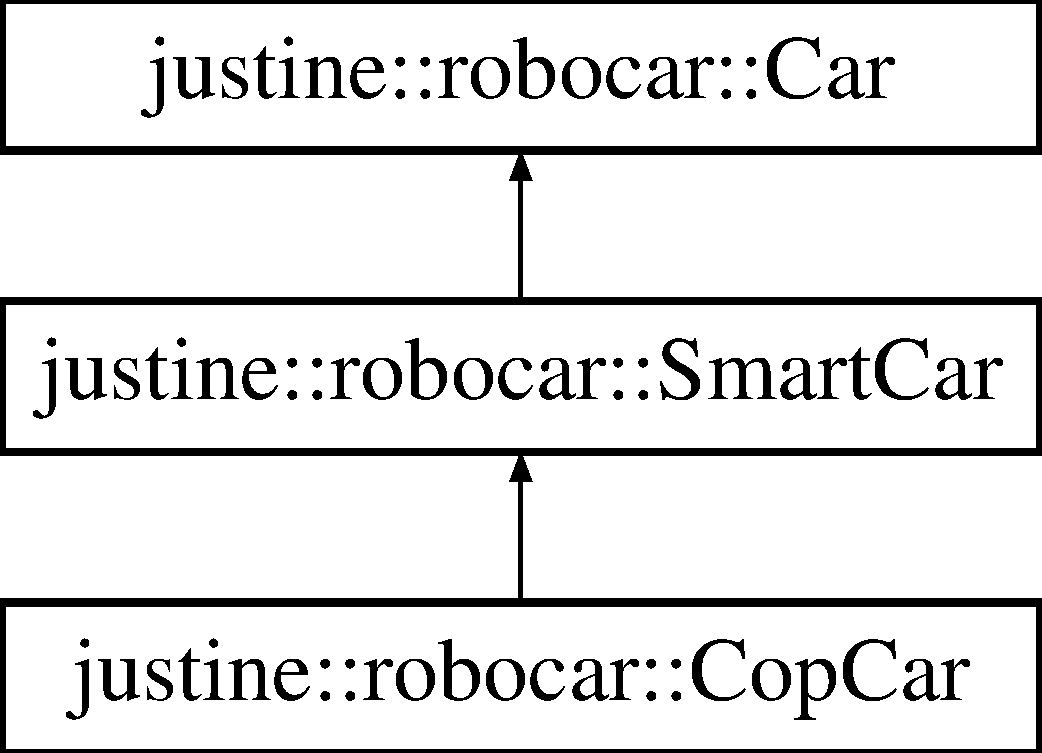
\includegraphics[height=3.000000cm]{classjustine_1_1robocar_1_1SmartCar}
\end{center}
\end{figure}
\subsection*{Public Member Functions}
\begin{DoxyCompactItemize}
\item 
\hypertarget{classjustine_1_1robocar_1_1SmartCar_af379e86c39a7f9ebc3642123782b4daa}{{\bfseries Smart\-Car} (\hyperlink{classjustine_1_1robocar_1_1Traffic}{Traffic} \&traffic, Car\-Type type, bool guided)}\label{classjustine_1_1robocar_1_1SmartCar_af379e86c39a7f9ebc3642123782b4daa}

\item 
\hypertarget{classjustine_1_1robocar_1_1SmartCar_a8702e16ac4bab30c1871997c934504b0}{virtual void {\bfseries step} ()}\label{classjustine_1_1robocar_1_1SmartCar_a8702e16ac4bab30c1871997c934504b0}

\item 
\hypertarget{classjustine_1_1robocar_1_1SmartCar_a507b7ccf9f989e3785a9a11828d49856}{virtual void {\bfseries init} ()}\label{classjustine_1_1robocar_1_1SmartCar_a507b7ccf9f989e3785a9a11828d49856}

\item 
\hypertarget{classjustine_1_1robocar_1_1SmartCar_a6d567bd88522d9bd592a8ad91b3e146e}{virtual void {\bfseries print} (std\-::ostream \&os) const }\label{classjustine_1_1robocar_1_1SmartCar_a6d567bd88522d9bd592a8ad91b3e146e}

\item 
\hypertarget{classjustine_1_1robocar_1_1SmartCar_a3b94461947ba83705444017958ef3cb3}{bool {\bfseries get\-\_\-guided} () const }\label{classjustine_1_1robocar_1_1SmartCar_a3b94461947ba83705444017958ef3cb3}

\item 
\hypertarget{classjustine_1_1robocar_1_1SmartCar_a2c1607a4bfe45e29f8a631b35e2f9a98}{bool {\bfseries set\-\_\-route} (std\-::vector$<$ unsigned int $>$ \&route)}\label{classjustine_1_1robocar_1_1SmartCar_a2c1607a4bfe45e29f8a631b35e2f9a98}

\item 
\hypertarget{classjustine_1_1robocar_1_1SmartCar_a8830e8b23885d3fb5039b7517cfa84dc}{virtual void {\bfseries next\-Edge} (void)}\label{classjustine_1_1robocar_1_1SmartCar_a8830e8b23885d3fb5039b7517cfa84dc}

\item 
\hypertarget{classjustine_1_1robocar_1_1SmartCar_a40947f44df0dcee308a6db4912d40646}{virtual void {\bfseries next\-Guided\-Edge} (void)}\label{classjustine_1_1robocar_1_1SmartCar_a40947f44df0dcee308a6db4912d40646}

\item 
\hypertarget{classjustine_1_1robocar_1_1SmartCar_a081cc666a87c18f0b7471f19c0afcdb0}{bool {\bfseries set\-\_\-fromto} (unsigned int from, unsigned int to)}\label{classjustine_1_1robocar_1_1SmartCar_a081cc666a87c18f0b7471f19c0afcdb0}

\end{DoxyCompactItemize}
\subsection*{Additional Inherited Members}


\subsection{Detailed Description}


Definition at line 163 of file car.\-hpp.



The documentation for this class was generated from the following files\-:\begin{DoxyCompactItemize}
\item 
src/\hyperlink{car_8hpp}{car.\-hpp}\item 
src/\hyperlink{car_8cpp}{car.\-cpp}\end{DoxyCompactItemize}

\hypertarget{classjustine_1_1robocar_1_1SmartCity}{\section{justine\-:\-:robocar\-:\-:Smart\-City Class Reference}
\label{classjustine_1_1robocar_1_1SmartCity}\index{justine\-::robocar\-::\-Smart\-City@{justine\-::robocar\-::\-Smart\-City}}
}
\subsection*{Public Member Functions}
\begin{DoxyCompactItemize}
\item 
\hypertarget{classjustine_1_1robocar_1_1SmartCity_aa9fee6663f3108a6f42171d011c7738d}{{\bfseries Smart\-City} (const char $\ast$osm\-\_\-file, const char $\ast$shm\-\_\-segment, const char $\ast$map\-\_\-file)}\label{classjustine_1_1robocar_1_1SmartCity_aa9fee6663f3108a6f42171d011c7738d}

\item 
\hypertarget{classjustine_1_1robocar_1_1SmartCity_a11a42f551adb2f030dcd788b1da210aa}{{\bfseries Smart\-City} (const char $\ast$osm\-\_\-file, const char $\ast$shm\-\_\-segment)}\label{classjustine_1_1robocar_1_1SmartCity_a11a42f551adb2f030dcd788b1da210aa}

\item 
\hypertarget{classjustine_1_1robocar_1_1SmartCity_a441ebb06a391b9c0409eb68751b15f43}{void {\bfseries processes} ()}\label{classjustine_1_1robocar_1_1SmartCity_a441ebb06a391b9c0409eb68751b15f43}

\item 
\hypertarget{classjustine_1_1robocar_1_1SmartCity_acafc9d2d447431798e32d1a652b2fe13}{virtual void {\bfseries city\-\_\-run} ()}\label{classjustine_1_1robocar_1_1SmartCity_acafc9d2d447431798e32d1a652b2fe13}

\item 
\hypertarget{classjustine_1_1robocar_1_1SmartCity_ad296267bfa7809696019064ed4a51432}{double \hyperlink{classjustine_1_1robocar_1_1SmartCity_ad296267bfa7809696019064ed4a51432}{bus\-Way\-Length} (bool verbose)}\label{classjustine_1_1robocar_1_1SmartCity_ad296267bfa7809696019064ed4a51432}

\begin{DoxyCompactList}\small\item\em This function gives a list of all the bus services operating in a given city. \end{DoxyCompactList}\end{DoxyCompactItemize}
\subsection*{Protected Attributes}
\begin{DoxyCompactItemize}
\item 
\hypertarget{classjustine_1_1robocar_1_1SmartCity_a4cdc70fa86d8bc7b71fc21eaaf640e06}{boost\-::interprocess\-::managed\-\_\-shared\-\_\-memory $\ast$ {\bfseries segment}}\label{classjustine_1_1robocar_1_1SmartCity_a4cdc70fa86d8bc7b71fc21eaaf640e06}

\item 
\hypertarget{classjustine_1_1robocar_1_1SmartCity_a1ddc2da8c48cde78087c4f49480cd013}{boost\-::interprocess\-::offset\-\_\-ptr\\*
$<$ shm\-\_\-map\-\_\-\-Type $>$ {\bfseries shm\-\_\-map}}\label{classjustine_1_1robocar_1_1SmartCity_a1ddc2da8c48cde78087c4f49480cd013}

\item 
\hypertarget{classjustine_1_1robocar_1_1SmartCity_abfe14f7488da07e158d10baa3d2ae48f}{int {\bfseries m\-\_\-delay} \{5000\}}\label{classjustine_1_1robocar_1_1SmartCity_abfe14f7488da07e158d10baa3d2ae48f}

\item 
\hypertarget{classjustine_1_1robocar_1_1SmartCity_a672c1f8a8550bff2f7c7f90f6ad09251}{bool {\bfseries m\-\_\-run} \{true\}}\label{classjustine_1_1robocar_1_1SmartCity_a672c1f8a8550bff2f7c7f90f6ad09251}

\end{DoxyCompactItemize}
\subsection*{Friends}
\begin{DoxyCompactItemize}
\item 
\hypertarget{classjustine_1_1robocar_1_1SmartCity_ac57d36e7cbaee1f2b1dd137e82a26cf9}{std\-::ostream \& {\bfseries operator$<$$<$} (std\-::ostream \&os, \hyperlink{classjustine_1_1robocar_1_1SmartCity}{Smart\-City} \&t)}\label{classjustine_1_1robocar_1_1SmartCity_ac57d36e7cbaee1f2b1dd137e82a26cf9}

\end{DoxyCompactItemize}


\subsection{Detailed Description}


Definition at line 83 of file smartcity.\-hpp.



The documentation for this class was generated from the following files\-:\begin{DoxyCompactItemize}
\item 
src/\hyperlink{smartcity_8hpp}{smartcity.\-hpp}\item 
src/smartcity.\-cpp\end{DoxyCompactItemize}

\hypertarget{classjustine_1_1robocar_1_1Traffic}{\section{justine\-:\-:robocar\-:\-:Traffic Class Reference}
\label{classjustine_1_1robocar_1_1Traffic}\index{justine\-::robocar\-::\-Traffic@{justine\-::robocar\-::\-Traffic}}
}
\subsection*{Public Member Functions}
\begin{DoxyCompactItemize}
\item 
\hypertarget{classjustine_1_1robocar_1_1Traffic_a8c17602b8a9ee0103d4b715bf6f86ace}{{\bfseries Traffic} (int size, const char $\ast$shm\-\_\-segment, double catchdist, Traffic\-Type type=Traffic\-Type\-::\-N\-O\-R\-M\-A\-L, int minutes=10)}\label{classjustine_1_1robocar_1_1Traffic_a8c17602b8a9ee0103d4b715bf6f86ace}

\item 
\hypertarget{classjustine_1_1robocar_1_1Traffic_abeaa22a436f4a41505edaca11720b228}{void {\bfseries processes} ()}\label{classjustine_1_1robocar_1_1Traffic_abeaa22a436f4a41505edaca11720b228}

\item 
\hypertarget{classjustine_1_1robocar_1_1Traffic_ace582f5edd9c7469e8926608ad7be6b6}{std\-::string {\bfseries get\-\_\-title} (std\-::string name)}\label{classjustine_1_1robocar_1_1Traffic_ace582f5edd9c7469e8926608ad7be6b6}

\item 
\hypertarget{classjustine_1_1robocar_1_1Traffic_ae35a8301f0c8596680386f640e8f0e88}{virtual \\*
osmium\-::unsigned\-\_\-object\-\_\-id\-\_\-type {\bfseries node} ()}\label{classjustine_1_1robocar_1_1Traffic_ae35a8301f0c8596680386f640e8f0e88}

\item 
\hypertarget{classjustine_1_1robocar_1_1Traffic_a1e7d6da5273c22994a958213931dc564}{virtual void {\bfseries traffic\-\_\-run} ()}\label{classjustine_1_1robocar_1_1Traffic_a1e7d6da5273c22994a958213931dc564}

\item 
\hypertarget{classjustine_1_1robocar_1_1Traffic_a29836a07c093bcfb3934167e61c3682c}{void {\bfseries steps} ()}\label{classjustine_1_1robocar_1_1Traffic_a29836a07c093bcfb3934167e61c3682c}

\item 
\hypertarget{classjustine_1_1robocar_1_1Traffic_a6b4911beb63b744d4d7a65a15544e74f}{void {\bfseries pursuit} (void)}\label{classjustine_1_1robocar_1_1Traffic_a6b4911beb63b744d4d7a65a15544e74f}

\item 
\hypertarget{classjustine_1_1robocar_1_1Traffic_a1e6eca609eadf0d0f1b9ad00bcbe4a42}{size\-\_\-t {\bfseries nedges} (osmium\-::unsigned\-\_\-object\-\_\-id\-\_\-type from) const }\label{classjustine_1_1robocar_1_1Traffic_a1e6eca609eadf0d0f1b9ad00bcbe4a42}

\item 
\hypertarget{classjustine_1_1robocar_1_1Traffic_a367916fb290fd78a172987778bb2cd48}{osmium\-::unsigned\-\_\-object\-\_\-id\-\_\-type {\bfseries alist} (osmium\-::unsigned\-\_\-object\-\_\-id\-\_\-type from, int to) const }\label{classjustine_1_1robocar_1_1Traffic_a367916fb290fd78a172987778bb2cd48}

\item 
\hypertarget{classjustine_1_1robocar_1_1Traffic_a515eddf0d41ed76ce292937d3e3b3b56}{int {\bfseries alist\-\_\-inv} (osmium\-::unsigned\-\_\-object\-\_\-id\-\_\-type from, osmium\-::unsigned\-\_\-object\-\_\-id\-\_\-type to) const }\label{classjustine_1_1robocar_1_1Traffic_a515eddf0d41ed76ce292937d3e3b3b56}

\item 
\hypertarget{classjustine_1_1robocar_1_1Traffic_aefa79e80cfa15f41b92ef83becdce4b4}{osmium\-::unsigned\-\_\-object\-\_\-id\-\_\-type {\bfseries salist} (osmium\-::unsigned\-\_\-object\-\_\-id\-\_\-type from, int to) const }\label{classjustine_1_1robocar_1_1Traffic_aefa79e80cfa15f41b92ef83becdce4b4}

\item 
\hypertarget{classjustine_1_1robocar_1_1Traffic_a57fdbe0f574bf9e717b6f08fed3b65d6}{void {\bfseries set\-\_\-salist} (osmium\-::unsigned\-\_\-object\-\_\-id\-\_\-type from, int to, osmium\-::unsigned\-\_\-object\-\_\-id\-\_\-type value)}\label{classjustine_1_1robocar_1_1Traffic_a57fdbe0f574bf9e717b6f08fed3b65d6}

\item 
\hypertarget{classjustine_1_1robocar_1_1Traffic_aff3732635f30a562dd868053181135f3}{osmium\-::unsigned\-\_\-object\-\_\-id\-\_\-type {\bfseries palist} (osmium\-::unsigned\-\_\-object\-\_\-id\-\_\-type from, int to) const }\label{classjustine_1_1robocar_1_1Traffic_aff3732635f30a562dd868053181135f3}

\item 
\hypertarget{classjustine_1_1robocar_1_1Traffic_a96423224fb3f375b03485d0f233ca845}{bool {\bfseries has\-Node} (osmium\-::unsigned\-\_\-object\-\_\-id\-\_\-type node)}\label{classjustine_1_1robocar_1_1Traffic_a96423224fb3f375b03485d0f233ca845}

\item 
\hypertarget{classjustine_1_1robocar_1_1Traffic_a17b14712edc48e8482c25480329df81e}{void {\bfseries start\-\_\-server} (boost\-::asio\-::io\-\_\-service \&io\-\_\-service, unsigned short port)}\label{classjustine_1_1robocar_1_1Traffic_a17b14712edc48e8482c25480329df81e}

\item 
\hypertarget{classjustine_1_1robocar_1_1Traffic_ae7328a945970421818d9440e10c83495}{void {\bfseries cmd\-\_\-session} (boost\-::asio\-::ip\-::tcp\-::socket sock)}\label{classjustine_1_1robocar_1_1Traffic_ae7328a945970421818d9440e10c83495}

\item 
\hypertarget{classjustine_1_1robocar_1_1Traffic_a887edf6621a3d7d1f05abcf2e1e6da98}{osmium\-::unsigned\-\_\-object\-\_\-id\-\_\-type {\bfseries naive\-\_\-node\-\_\-for\-\_\-nearest\-\_\-gangster} (osmium\-::unsigned\-\_\-object\-\_\-id\-\_\-type from, osmium\-::unsigned\-\_\-object\-\_\-id\-\_\-type to, osmium\-::unsigned\-\_\-object\-\_\-id\-\_\-type step)}\label{classjustine_1_1robocar_1_1Traffic_a887edf6621a3d7d1f05abcf2e1e6da98}

\item 
\hypertarget{classjustine_1_1robocar_1_1Traffic_a362e2f333db32dde70f4514852bec749}{double {\bfseries dst} (osmium\-::unsigned\-\_\-object\-\_\-id\-\_\-type n1, osmium\-::unsigned\-\_\-object\-\_\-id\-\_\-type n2) const }\label{classjustine_1_1robocar_1_1Traffic_a362e2f333db32dde70f4514852bec749}

\item 
\hypertarget{classjustine_1_1robocar_1_1Traffic_adf624af90c5f83fafaf81d246258ba33}{double {\bfseries dst} (double lon1, double lat1, double lon2, double lat2) const }\label{classjustine_1_1robocar_1_1Traffic_adf624af90c5f83fafaf81d246258ba33}

\item 
\hypertarget{classjustine_1_1robocar_1_1Traffic_a49503774701cc98b36ceb82d81c2e3c1}{void {\bfseries to\-G\-P\-S} (osmium\-::unsigned\-\_\-object\-\_\-id\-\_\-type from, osmium\-::unsigned\-\_\-object\-\_\-id\-\_\-type to, osmium\-::unsigned\-\_\-object\-\_\-id\-\_\-type step, double $\ast$lo, double $\ast$la) const }\label{classjustine_1_1robocar_1_1Traffic_a49503774701cc98b36ceb82d81c2e3c1}

\item 
\hypertarget{classjustine_1_1robocar_1_1Traffic_accd02fdbc9ed06dafaef1644ba5ca38f}{osmium\-::unsigned\-\_\-object\-\_\-id\-\_\-type {\bfseries naive\-\_\-nearest\-\_\-gangster} (osmium\-::unsigned\-\_\-object\-\_\-id\-\_\-type from, osmium\-::unsigned\-\_\-object\-\_\-id\-\_\-type to, osmium\-::unsigned\-\_\-object\-\_\-id\-\_\-type step)}\label{classjustine_1_1robocar_1_1Traffic_accd02fdbc9ed06dafaef1644ba5ca38f}

\item 
\hypertarget{classjustine_1_1robocar_1_1Traffic_a77d713d1e1512c19d4aa491d42489c4b}{Traffic\-Type {\bfseries get\-\_\-type} () const }\label{classjustine_1_1robocar_1_1Traffic_a77d713d1e1512c19d4aa491d42489c4b}

\item 
\hypertarget{classjustine_1_1robocar_1_1Traffic_a8c61ac39493e46faaa4f3f3025241300}{int {\bfseries get\-\_\-time} () const }\label{classjustine_1_1robocar_1_1Traffic_a8c61ac39493e46faaa4f3f3025241300}

\end{DoxyCompactItemize}
\subsection*{Protected Attributes}
\begin{DoxyCompactItemize}
\item 
\hypertarget{classjustine_1_1robocar_1_1Traffic_a49d195915f7de5e8e05b878d52d0e18a}{boost\-::interprocess\-::managed\-\_\-shared\-\_\-memory $\ast$ {\bfseries segment}}\label{classjustine_1_1robocar_1_1Traffic_a49d195915f7de5e8e05b878d52d0e18a}

\item 
\hypertarget{classjustine_1_1robocar_1_1Traffic_ad7b1accb32b08e53e1e87de54d47ca36}{boost\-::interprocess\-::offset\-\_\-ptr\\*
$<$ shm\-\_\-map\-\_\-\-Type $>$ {\bfseries shm\-\_\-map}}\label{classjustine_1_1robocar_1_1Traffic_ad7b1accb32b08e53e1e87de54d47ca36}

\item 
\hypertarget{classjustine_1_1robocar_1_1Traffic_aafdd2b06902033f70bc2d9fab7a7ac9a}{int {\bfseries m\-\_\-delay} \{200\}}\label{classjustine_1_1robocar_1_1Traffic_aafdd2b06902033f70bc2d9fab7a7ac9a}

\item 
\hypertarget{classjustine_1_1robocar_1_1Traffic_a5e2d2ac702682e5190c163e1fbfedd11}{bool {\bfseries m\-\_\-run} \{true\}}\label{classjustine_1_1robocar_1_1Traffic_a5e2d2ac702682e5190c163e1fbfedd11}

\item 
\hypertarget{classjustine_1_1robocar_1_1Traffic_ae2962840b6cf17cab957c2b7a2ebe675}{double {\bfseries m\-\_\-catchdist} \{15.\-5\}}\label{classjustine_1_1robocar_1_1Traffic_ae2962840b6cf17cab957c2b7a2ebe675}

\end{DoxyCompactItemize}
\subsection*{Friends}
\begin{DoxyCompactItemize}
\item 
\hypertarget{classjustine_1_1robocar_1_1Traffic_adecf1b9bb1d67626720d29b0bae104fb}{std\-::ostream \& {\bfseries operator$<$$<$} (std\-::ostream \&os, \hyperlink{classjustine_1_1robocar_1_1Traffic}{Traffic} \&t)}\label{classjustine_1_1robocar_1_1Traffic_adecf1b9bb1d67626720d29b0bae104fb}

\end{DoxyCompactItemize}


\subsection{Detailed Description}


Definition at line 81 of file traffic.\-hpp.



The documentation for this class was generated from the following files\-:\begin{DoxyCompactItemize}
\item 
src/traffic.\-hpp\item 
src/\hyperlink{traffic_8cpp}{traffic.\-cpp}\end{DoxyCompactItemize}

\hypertarget{structyy__buffer__state}{\section{yy\-\_\-buffer\-\_\-state Struct Reference}
\label{structyy__buffer__state}\index{yy\-\_\-buffer\-\_\-state@{yy\-\_\-buffer\-\_\-state}}
}
\subsection*{Public Attributes}
\begin{DoxyCompactItemize}
\item 
\hypertarget{structyy__buffer__state_a3cea2f85a5c18fae4a8dd1ca44c3a977}{std\-::istream $\ast$ {\bfseries yy\-\_\-input\-\_\-file}}\label{structyy__buffer__state_a3cea2f85a5c18fae4a8dd1ca44c3a977}

\item 
\hypertarget{structyy__buffer__state_ad7b8df8d8a4688e57b0b8d3ca75adc85}{char $\ast$ {\bfseries yy\-\_\-ch\-\_\-buf}}\label{structyy__buffer__state_ad7b8df8d8a4688e57b0b8d3ca75adc85}

\item 
\hypertarget{structyy__buffer__state_a58aa927f098b99d99e75da80f9b681ef}{char $\ast$ {\bfseries yy\-\_\-buf\-\_\-pos}}\label{structyy__buffer__state_a58aa927f098b99d99e75da80f9b681ef}

\item 
\hypertarget{structyy__buffer__state_a48302f5f3477a9c78bbddf56d356ef54}{yy\-\_\-size\-\_\-t {\bfseries yy\-\_\-buf\-\_\-size}}\label{structyy__buffer__state_a48302f5f3477a9c78bbddf56d356ef54}

\item 
\hypertarget{structyy__buffer__state_a06406208824817acfec2183b79080945}{int {\bfseries yy\-\_\-n\-\_\-chars}}\label{structyy__buffer__state_a06406208824817acfec2183b79080945}

\item 
\hypertarget{structyy__buffer__state_a80ce2431c70dc4f89ced487f18449465}{int {\bfseries yy\-\_\-is\-\_\-our\-\_\-buffer}}\label{structyy__buffer__state_a80ce2431c70dc4f89ced487f18449465}

\item 
\hypertarget{structyy__buffer__state_abf5c70eea75581b58c0ee7bd31b14490}{int {\bfseries yy\-\_\-is\-\_\-interactive}}\label{structyy__buffer__state_abf5c70eea75581b58c0ee7bd31b14490}

\item 
\hypertarget{structyy__buffer__state_a9d60c60af6e1a6f69de16871fd64f85f}{int {\bfseries yy\-\_\-at\-\_\-bol}}\label{structyy__buffer__state_a9d60c60af6e1a6f69de16871fd64f85f}

\item 
int \hyperlink{structyy__buffer__state_a818e94bc9c766e683c60df1e9fd01199}{yy\-\_\-bs\-\_\-lineno}
\item 
int \hyperlink{structyy__buffer__state_a10c4fcd8be759e6bf11e6d3e8cdb0307}{yy\-\_\-bs\-\_\-column}
\item 
\hypertarget{structyy__buffer__state_a63d2afbb1d79a3fc63df9e12626f827d}{int {\bfseries yy\-\_\-fill\-\_\-buffer}}\label{structyy__buffer__state_a63d2afbb1d79a3fc63df9e12626f827d}

\item 
\hypertarget{structyy__buffer__state_a70fd925d37a2f0454fbd0def675d106c}{int {\bfseries yy\-\_\-buffer\-\_\-status}}\label{structyy__buffer__state_a70fd925d37a2f0454fbd0def675d106c}

\end{DoxyCompactItemize}


\subsection{Detailed Description}


Definition at line 208 of file carlexer.\-cc.



\subsection{Member Data Documentation}
\hypertarget{structyy__buffer__state_a10c4fcd8be759e6bf11e6d3e8cdb0307}{\index{yy\-\_\-buffer\-\_\-state@{yy\-\_\-buffer\-\_\-state}!yy\-\_\-bs\-\_\-column@{yy\-\_\-bs\-\_\-column}}
\index{yy\-\_\-bs\-\_\-column@{yy\-\_\-bs\-\_\-column}!yy_buffer_state@{yy\-\_\-buffer\-\_\-state}}
\subsubsection[{yy\-\_\-bs\-\_\-column}]{\setlength{\rightskip}{0pt plus 5cm}int yy\-\_\-buffer\-\_\-state\-::yy\-\_\-bs\-\_\-column}}\label{structyy__buffer__state_a10c4fcd8be759e6bf11e6d3e8cdb0307}
The column count. 

Definition at line 246 of file carlexer.\-cc.

\hypertarget{structyy__buffer__state_a818e94bc9c766e683c60df1e9fd01199}{\index{yy\-\_\-buffer\-\_\-state@{yy\-\_\-buffer\-\_\-state}!yy\-\_\-bs\-\_\-lineno@{yy\-\_\-bs\-\_\-lineno}}
\index{yy\-\_\-bs\-\_\-lineno@{yy\-\_\-bs\-\_\-lineno}!yy_buffer_state@{yy\-\_\-buffer\-\_\-state}}
\subsubsection[{yy\-\_\-bs\-\_\-lineno}]{\setlength{\rightskip}{0pt plus 5cm}int yy\-\_\-buffer\-\_\-state\-::yy\-\_\-bs\-\_\-lineno}}\label{structyy__buffer__state_a818e94bc9c766e683c60df1e9fd01199}
The line count. 

Definition at line 245 of file carlexer.\-cc.



The documentation for this struct was generated from the following file\-:\begin{DoxyCompactItemize}
\item 
src/carlexer.\-cc\end{DoxyCompactItemize}

\hypertarget{structyy__trans__info}{\section{yy\-\_\-trans\-\_\-info Struct Reference}
\label{structyy__trans__info}\index{yy\-\_\-trans\-\_\-info@{yy\-\_\-trans\-\_\-info}}
}
\subsection*{Public Attributes}
\begin{DoxyCompactItemize}
\item 
\hypertarget{structyy__trans__info_a5c9f61e770deef50bd4e697310342fe9}{flex\-\_\-int32\-\_\-t {\bfseries yy\-\_\-verify}}\label{structyy__trans__info_a5c9f61e770deef50bd4e697310342fe9}

\item 
\hypertarget{structyy__trans__info_ae0715250c2bef261e596e77e0030f13e}{flex\-\_\-int32\-\_\-t {\bfseries yy\-\_\-nxt}}\label{structyy__trans__info_ae0715250c2bef261e596e77e0030f13e}

\end{DoxyCompactItemize}


\subsection{Detailed Description}


Definition at line 341 of file carlexer.\-cc.



The documentation for this struct was generated from the following file\-:\begin{DoxyCompactItemize}
\item 
src/carlexer.\-cc\end{DoxyCompactItemize}

\chapter{File Documentation}
\hypertarget{car_8cpp}{\section{src/car.cpp File Reference}
\label{car_8cpp}\index{src/car.\-cpp@{src/car.\-cpp}}
}


Justine -\/ this is a rapid prototype for development of Robocar City Emulator.  


{\ttfamily \#include $<$car.\-hpp$>$}\\*
{\ttfamily \#include $<$traffic.\-hpp$>$}\\*
{\ttfamily \#include $<$boost/iterator/iterator\-\_\-concepts.\-hpp$>$}\\*


\subsection{Detailed Description}
Justine -\/ this is a rapid prototype for development of Robocar City Emulator. \begin{DoxyAuthor}{Author}
Norbert Bátfai \href{mailto:nbatfai@gmail.com}{\tt nbatfai@gmail.\-com} 
\end{DoxyAuthor}
\begin{DoxyVersion}{Version}
0.\-0.\-10
\end{DoxyVersion}
\hypertarget{traffic_8cpp_LICENSE}{}\subsection{L\-I\-C\-E\-N\-S\-E}\label{traffic_8cpp_LICENSE}
Copyright (C) 2014 Norbert Bátfai, \href{mailto:batfai.norbert@inf.unideb.hu}{\tt batfai.\-norbert@inf.\-unideb.\-hu}

This program is free software\-: you can redistribute it and/or modify it under the terms of the G\-N\-U General Public License as published by the Free Software Foundation, either version 3 of the License, or (at your option) any later version.

This program is distributed in the hope that it will be useful, but W\-I\-T\-H\-O\-U\-T A\-N\-Y W\-A\-R\-R\-A\-N\-T\-Y; without even the implied warranty of M\-E\-R\-C\-H\-A\-N\-T\-A\-B\-I\-L\-I\-T\-Y or F\-I\-T\-N\-E\-S\-S F\-O\-R A P\-A\-R\-T\-I\-C\-U\-L\-A\-R P\-U\-R\-P\-O\-S\-E. See the G\-N\-U General Public License for more details.

You should have received a copy of the G\-N\-U General Public License along with this program. If not, see \href{http://www.gnu.org/licenses/}{\tt http\-://www.\-gnu.\-org/licenses/}.\hypertarget{traffic_8cpp_DESCRIPTION}{}\subsection{D\-E\-S\-C\-R\-I\-P\-T\-I\-O\-N}\label{traffic_8cpp_DESCRIPTION}
Robocar City Emulator and Robocar World Championship

desc 

Definition in file \hyperlink{car_8cpp_source}{car.\-cpp}.


\hypertarget{car_8hpp}{\section{src/car.hpp File Reference}
\label{car_8hpp}\index{src/car.\-hpp@{src/car.\-hpp}}
}


Justine -\/ this is a rapid prototype for development of Robocar City Emulator.  


{\ttfamily \#include $<$osmium/osm/types.\-hpp$>$}\\*
{\ttfamily \#include $<$iostream$>$}\\*
{\ttfamily \#include $<$vector$>$}\\*
{\ttfamily \#include $<$osmreader.\-hpp$>$}\\*
{\ttfamily \#include $<$algorithm$>$}\\*
\subsection*{Classes}
\begin{DoxyCompactItemize}
\item 
class \hyperlink{classjustine_1_1robocar_1_1Car}{justine\-::robocar\-::\-Car}
\item 
class \hyperlink{classjustine_1_1robocar_1_1AntCar}{justine\-::robocar\-::\-Ant\-Car}
\item 
class \hyperlink{classjustine_1_1robocar_1_1SmartCar}{justine\-::robocar\-::\-Smart\-Car}
\item 
class \hyperlink{classjustine_1_1robocar_1_1CopCar}{justine\-::robocar\-::\-Cop\-Car}
\end{DoxyCompactItemize}
\subsection*{Enumerations}
\begin{DoxyCompactItemize}
\item 
enum {\bfseries Car\-Type} \-: unsigned int \{ {\bfseries N\-O\-R\-M\-A\-L} =0, 
{\bfseries P\-O\-L\-I\-C\-E}, 
{\bfseries G\-A\-N\-G\-S\-T\-E\-R}, 
{\bfseries C\-A\-U\-G\-H\-T}
 \}
\end{DoxyCompactItemize}


\subsection{Detailed Description}
Justine -\/ this is a rapid prototype for development of Robocar City Emulator. \begin{DoxyAuthor}{Author}
Norbert Bátfai \href{mailto:nbatfai@gmail.com}{\tt nbatfai@gmail.\-com} 
\end{DoxyAuthor}
\begin{DoxyVersion}{Version}
0.\-0.\-10
\end{DoxyVersion}
\hypertarget{traffic_8cpp_LICENSE}{}\subsection{L\-I\-C\-E\-N\-S\-E}\label{traffic_8cpp_LICENSE}
Copyright (C) 2014 Norbert Bátfai, \href{mailto:batfai.norbert@inf.unideb.hu}{\tt batfai.\-norbert@inf.\-unideb.\-hu}

This program is free software\-: you can redistribute it and/or modify it under the terms of the G\-N\-U General Public License as published by the Free Software Foundation, either version 3 of the License, or (at your option) any later version.

This program is distributed in the hope that it will be useful, but W\-I\-T\-H\-O\-U\-T A\-N\-Y W\-A\-R\-R\-A\-N\-T\-Y; without even the implied warranty of M\-E\-R\-C\-H\-A\-N\-T\-A\-B\-I\-L\-I\-T\-Y or F\-I\-T\-N\-E\-S\-S F\-O\-R A P\-A\-R\-T\-I\-C\-U\-L\-A\-R P\-U\-R\-P\-O\-S\-E. See the G\-N\-U General Public License for more details.

You should have received a copy of the G\-N\-U General Public License along with this program. If not, see \href{http://www.gnu.org/licenses/}{\tt http\-://www.\-gnu.\-org/licenses/}.\hypertarget{traffic_8cpp_DESCRIPTION}{}\subsection{D\-E\-S\-C\-R\-I\-P\-T\-I\-O\-N}\label{traffic_8cpp_DESCRIPTION}
Robocar City Emulator and Robocar World Championship

desc 

Definition in file \hyperlink{car_8hpp_source}{car.\-hpp}.


\hypertarget{carlexer_8hpp}{\section{src/carlexer.hpp File Reference}
\label{carlexer_8hpp}\index{src/carlexer.\-hpp@{src/carlexer.\-hpp}}
}


Justine -\/ this is a rapid prototype for development of Robocar City Emulator.  


{\ttfamily \#include $<$Flex\-Lexer.\-h$>$}\\*
{\ttfamily \#include $<$iostream$>$}\\*
{\ttfamily \#include $<$sstream$>$}\\*
{\ttfamily \#include $<$cstring$>$}\\*
{\ttfamily \#include $<$cstdio$>$}\\*
{\ttfamily \#include $<$vector$>$}\\*
\subsection*{Classes}
\begin{DoxyCompactItemize}
\item 
class \hyperlink{classjustine_1_1robocar_1_1CarLexer}{justine\-::robocar\-::\-Car\-Lexer}
\end{DoxyCompactItemize}


\subsection{Detailed Description}
Justine -\/ this is a rapid prototype for development of Robocar City Emulator. \begin{DoxyAuthor}{Author}
Norbert Bátfai \href{mailto:nbatfai@gmail.com}{\tt nbatfai@gmail.\-com} 
\end{DoxyAuthor}
\begin{DoxyVersion}{Version}
0.\-0.\-10
\end{DoxyVersion}
\hypertarget{traffic_8cpp_LICENSE}{}\subsection{L\-I\-C\-E\-N\-S\-E}\label{traffic_8cpp_LICENSE}
Copyright (C) 2014 Norbert Bátfai, \href{mailto:batfai.norbert@inf.unideb.hu}{\tt batfai.\-norbert@inf.\-unideb.\-hu}

This program is free software\-: you can redistribute it and/or modify it under the terms of the G\-N\-U General Public License as published by the Free Software Foundation, either version 3 of the License, or (at your option) any later version.

This program is distributed in the hope that it will be useful, but W\-I\-T\-H\-O\-U\-T A\-N\-Y W\-A\-R\-R\-A\-N\-T\-Y; without even the implied warranty of M\-E\-R\-C\-H\-A\-N\-T\-A\-B\-I\-L\-I\-T\-Y or F\-I\-T\-N\-E\-S\-S F\-O\-R A P\-A\-R\-T\-I\-C\-U\-L\-A\-R P\-U\-R\-P\-O\-S\-E. See the G\-N\-U General Public License for more details.

You should have received a copy of the G\-N\-U General Public License along with this program. If not, see \href{http://www.gnu.org/licenses/}{\tt http\-://www.\-gnu.\-org/licenses/}.\hypertarget{traffic_8cpp_DESCRIPTION}{}\subsection{D\-E\-S\-C\-R\-I\-P\-T\-I\-O\-N}\label{traffic_8cpp_DESCRIPTION}
Robocar City Emulator and Robocar World Championship

desc 

Definition in file \hyperlink{carlexer_8hpp_source}{carlexer.\-hpp}.


\hypertarget{mainpage_8h}{\section{src/mainpage.h File Reference}
\label{mainpage_8h}\index{src/mainpage.\-h@{src/mainpage.\-h}}
}


Justine -\/ this is a rapid prototype for development of Robocar City Emulator.  




\subsection{Detailed Description}
Justine -\/ this is a rapid prototype for development of Robocar City Emulator. \begin{DoxyAuthor}{Author}
Norbert Bátfai \href{mailto:nbatfai@gmail.com}{\tt nbatfai@gmail.\-com} 
\end{DoxyAuthor}


Definition in file \hyperlink{mainpage_8h_source}{mainpage.\-h}.


\hypertarget{myshmclient-main_8cpp}{\section{src/myshmclient-\/main.cpp File Reference}
\label{myshmclient-main_8cpp}\index{src/myshmclient-\/main.\-cpp@{src/myshmclient-\/main.\-cpp}}
}


Justine -\/ this is a rapid prototype for development of Robocar City Emulator.  


{\ttfamily \#include $<$myshmclient.\-hpp$>$}\\*
{\ttfamily \#include $<$boost/program\-\_\-options.\-hpp$>$}\\*
\subsection*{Functions}
\begin{DoxyCompactItemize}
\item 
\hypertarget{myshmclient-main_8cpp_a0ddf1224851353fc92bfbff6f499fa97}{int {\bfseries main} (int argc, char $\ast$argv\mbox{[}$\,$\mbox{]})}\label{myshmclient-main_8cpp_a0ddf1224851353fc92bfbff6f499fa97}

\end{DoxyCompactItemize}


\subsection{Detailed Description}
Justine -\/ this is a rapid prototype for development of Robocar City Emulator. \begin{DoxyAuthor}{Author}
Norbert Bátfai \href{mailto:nbatfai@gmail.com}{\tt nbatfai@gmail.\-com} 
\end{DoxyAuthor}
\begin{DoxyVersion}{Version}
0.\-0.\-10
\end{DoxyVersion}
\hypertarget{traffic_8cpp_LICENSE}{}\subsection{L\-I\-C\-E\-N\-S\-E}\label{traffic_8cpp_LICENSE}
Copyright (C) 2014 Norbert Bátfai, \href{mailto:batfai.norbert@inf.unideb.hu}{\tt batfai.\-norbert@inf.\-unideb.\-hu}

This program is free software\-: you can redistribute it and/or modify it under the terms of the G\-N\-U General Public License as published by the Free Software Foundation, either version 3 of the License, or (at your option) any later version.

This program is distributed in the hope that it will be useful, but W\-I\-T\-H\-O\-U\-T A\-N\-Y W\-A\-R\-R\-A\-N\-T\-Y; without even the implied warranty of M\-E\-R\-C\-H\-A\-N\-T\-A\-B\-I\-L\-I\-T\-Y or F\-I\-T\-N\-E\-S\-S F\-O\-R A P\-A\-R\-T\-I\-C\-U\-L\-A\-R P\-U\-R\-P\-O\-S\-E. See the G\-N\-U General Public License for more details.

You should have received a copy of the G\-N\-U General Public License along with this program. If not, see \href{http://www.gnu.org/licenses/}{\tt http\-://www.\-gnu.\-org/licenses/}.\hypertarget{traffic_8cpp_DESCRIPTION}{}\subsection{D\-E\-S\-C\-R\-I\-P\-T\-I\-O\-N}\label{traffic_8cpp_DESCRIPTION}
Robocar City Emulator and Robocar World Championship

desc 

Definition in file \hyperlink{myshmclient-main_8cpp_source}{myshmclient-\/main.\-cpp}.


\hypertarget{myshmclient_8cpp}{\section{src/myshmclient.cpp File Reference}
\label{myshmclient_8cpp}\index{src/myshmclient.\-cpp@{src/myshmclient.\-cpp}}
}


Justine -\/ this is a rapid prototype for development of Robocar City Emulator.  


{\ttfamily \#include $<$myshmclient.\-hpp$>$}\\*
\subsection*{Variables}
\begin{DoxyCompactItemize}
\item 
\hypertarget{myshmclient_8cpp_aef0fac4c91056db502c9292d5f5a0c35}{char {\bfseries data} \mbox{[}524288\mbox{]}}\label{myshmclient_8cpp_aef0fac4c91056db502c9292d5f5a0c35}

\end{DoxyCompactItemize}


\subsection{Detailed Description}
Justine -\/ this is a rapid prototype for development of Robocar City Emulator. \begin{DoxyAuthor}{Author}
Norbert Bátfai \href{mailto:nbatfai@gmail.com}{\tt nbatfai@gmail.\-com} 
\end{DoxyAuthor}
\begin{DoxyVersion}{Version}
0.\-0.\-10
\end{DoxyVersion}
\hypertarget{traffic_8cpp_LICENSE}{}\subsection{L\-I\-C\-E\-N\-S\-E}\label{traffic_8cpp_LICENSE}
Copyright (C) 2014 Norbert Bátfai, \href{mailto:batfai.norbert@inf.unideb.hu}{\tt batfai.\-norbert@inf.\-unideb.\-hu}

This program is free software\-: you can redistribute it and/or modify it under the terms of the G\-N\-U General Public License as published by the Free Software Foundation, either version 3 of the License, or (at your option) any later version.

This program is distributed in the hope that it will be useful, but W\-I\-T\-H\-O\-U\-T A\-N\-Y W\-A\-R\-R\-A\-N\-T\-Y; without even the implied warranty of M\-E\-R\-C\-H\-A\-N\-T\-A\-B\-I\-L\-I\-T\-Y or F\-I\-T\-N\-E\-S\-S F\-O\-R A P\-A\-R\-T\-I\-C\-U\-L\-A\-R P\-U\-R\-P\-O\-S\-E. See the G\-N\-U General Public License for more details.

You should have received a copy of the G\-N\-U General Public License along with this program. If not, see \href{http://www.gnu.org/licenses/}{\tt http\-://www.\-gnu.\-org/licenses/}.\hypertarget{traffic_8cpp_DESCRIPTION}{}\subsection{D\-E\-S\-C\-R\-I\-P\-T\-I\-O\-N}\label{traffic_8cpp_DESCRIPTION}
Robocar City Emulator and Robocar World Championship

desc 

Definition in file \hyperlink{myshmclient_8cpp_source}{myshmclient.\-cpp}.


\hypertarget{myshmclient_8hpp}{\section{src/myshmclient.hpp File Reference}
\label{myshmclient_8hpp}\index{src/myshmclient.\-hpp@{src/myshmclient.\-hpp}}
}


Justine -\/ this is a rapid prototype for development of Robocar City Emulator.  


{\ttfamily \#include $<$boost/interprocess/managed\-\_\-shared\-\_\-memory.\-hpp$>$}\\*
{\ttfamily \#include $<$boost/interprocess/allocators/allocator.\-hpp$>$}\\*
{\ttfamily \#include $<$boost/interprocess/containers/map.\-hpp$>$}\\*
{\ttfamily \#include $<$boost/interprocess/containers/vector.\-hpp$>$}\\*
{\ttfamily \#include $<$boost/interprocess/containers/string.\-hpp$>$}\\*
{\ttfamily \#include $<$smartcity.\-hpp$>$}\\*
{\ttfamily \#include $<$car.\-hpp$>$}\\*
{\ttfamily \#include $<$cstdlib$>$}\\*
{\ttfamily \#include $<$iterator$>$}\\*
{\ttfamily \#include $<$boost/asio.\-hpp$>$}\\*
{\ttfamily \#include $<$limits$>$}\\*
{\ttfamily \#include $<$memory$>$}\\*
{\ttfamily \#include $<$boost/graph/adjacency\-\_\-list.\-hpp$>$}\\*
{\ttfamily \#include $<$boost/graph/graph\-\_\-traits.\-hpp$>$}\\*
{\ttfamily \#include $<$boost/graph/dijkstra\-\_\-shortest\-\_\-paths.\-hpp$>$}\\*
{\ttfamily \#include $<$boost/graph/properties.\-hpp$>$}\\*
{\ttfamily \#include $<$boost/property\-\_\-map/property\-\_\-map.\-hpp$>$}\\*
{\ttfamily \#include $<$shmclient.\-hpp$>$}\\*
{\ttfamily \#include $<$algorithm$>$}\\*
{\ttfamily \#include $<$boost/graph/bellman\-\_\-ford\-\_\-shortest\-\_\-paths.\-hpp$>$}\\*
{\ttfamily \#include $<$boost/graph/graphviz.\-hpp$>$}\\*
{\ttfamily \#include $<$fstream$>$}\\*
\subsection*{Classes}
\begin{DoxyCompactItemize}
\item 
class \hyperlink{classjustine_1_1sampleclient_1_1MyShmClient}{justine\-::sampleclient\-::\-My\-Shm\-Client}
\begin{DoxyCompactList}\small\item\em A sample class used for testing the routing algorithms. \end{DoxyCompactList}\end{DoxyCompactItemize}
\subsection*{Typedefs}
\begin{DoxyCompactItemize}
\item 
\hypertarget{namespacejustine_1_1sampleclient_ab228342eb20e9184cef6b072b1508058}{typedef boost\-::adjacency\-\_\-list\\*
$<$ boost\-::list\-S, boost\-::vec\-S, \\*
boost\-::directed\-S, \\*
boost\-::property\\*
$<$ boost\-::vertex\-\_\-name\-\_\-t, \\*
osmium\-::unsigned\-\_\-object\-\_\-id\-\_\-type $>$\\*
, boost\-::property\\*
$<$ boost\-::edge\-\_\-weight\-\_\-t, int $>$ $>$ {\bfseries justine\-::sampleclient\-::\-Node\-Ref\-Graph}}\label{namespacejustine_1_1sampleclient_ab228342eb20e9184cef6b072b1508058}

\item 
\hypertarget{namespacejustine_1_1sampleclient_a13656221ca660ae4edca6b135920b4c0}{typedef boost\-::graph\-\_\-traits\\*
$<$ Node\-Ref\-Graph $>$\\*
\-::vertex\-\_\-descriptor {\bfseries justine\-::sampleclient\-::\-N\-R\-G\-Vertex}}\label{namespacejustine_1_1sampleclient_a13656221ca660ae4edca6b135920b4c0}

\item 
\hypertarget{namespacejustine_1_1sampleclient_ade1a2d36ccfed17fef2dbfa78f1a21ce}{typedef boost\-::graph\-\_\-traits\\*
$<$ Node\-Ref\-Graph $>$\\*
\-::vertex\-\_\-iterator {\bfseries justine\-::sampleclient\-::\-N\-R\-G\-Vertex\-Iter}}\label{namespacejustine_1_1sampleclient_ade1a2d36ccfed17fef2dbfa78f1a21ce}

\item 
\hypertarget{namespacejustine_1_1sampleclient_a3840a294abd9a737842de7521a98ff04}{typedef boost\-::graph\-\_\-traits\\*
$<$ Node\-Ref\-Graph $>$\\*
\-::edge\-\_\-descriptor {\bfseries justine\-::sampleclient\-::\-N\-R\-G\-Edge}}\label{namespacejustine_1_1sampleclient_a3840a294abd9a737842de7521a98ff04}

\item 
\hypertarget{namespacejustine_1_1sampleclient_a3040f83f7157a83f52921523b876ec3e}{typedef boost\-::graph\-\_\-traits\\*
$<$ Node\-Ref\-Graph $>$\\*
\-::edge\-\_\-iterator {\bfseries justine\-::sampleclient\-::\-N\-R\-G\-Edge\-Iter}}\label{namespacejustine_1_1sampleclient_a3040f83f7157a83f52921523b876ec3e}

\item 
\hypertarget{namespacejustine_1_1sampleclient_afc57a783f10c45fbeccfe899476f99b2}{typedef boost\-::property\-\_\-map\\*
$<$ Node\-Ref\-Graph, \\*
boost\-::vertex\-\_\-name\-\_\-t $>$\-::type {\bfseries justine\-::sampleclient\-::\-Vertex\-Name\-Map}}\label{namespacejustine_1_1sampleclient_afc57a783f10c45fbeccfe899476f99b2}

\item 
\hypertarget{namespacejustine_1_1sampleclient_a923cb4a7a69c7182397fa18742651509}{typedef boost\-::property\-\_\-map\\*
$<$ Node\-Ref\-Graph, \\*
boost\-::vertex\-\_\-index\-\_\-t $>$\-::type {\bfseries justine\-::sampleclient\-::\-Vertex\-Index\-Map}}\label{namespacejustine_1_1sampleclient_a923cb4a7a69c7182397fa18742651509}

\item 
\hypertarget{namespacejustine_1_1sampleclient_ad6dd9571f36d9b2e3dcbf768e6407f27}{typedef \\*
boost\-::iterator\-\_\-property\-\_\-map\\*
$<$ N\-R\-G\-Vertex $\ast$, Vertex\-Index\-Map, \\*
N\-R\-G\-Vertex, N\-R\-G\-Vertex \& $>$ {\bfseries justine\-::sampleclient\-::\-Predecessor\-Map}}\label{namespacejustine_1_1sampleclient_ad6dd9571f36d9b2e3dcbf768e6407f27}

\item 
\hypertarget{namespacejustine_1_1sampleclient_aa10b4de83c32c463b872b1e78ab28a1c}{typedef \\*
boost\-::iterator\-\_\-property\-\_\-map\\*
$<$ int $\ast$, Vertex\-Index\-Map, int, \\*
int \& $>$ {\bfseries justine\-::sampleclient\-::\-Distance\-Map}}\label{namespacejustine_1_1sampleclient_aa10b4de83c32c463b872b1e78ab28a1c}

\item 
\hypertarget{namespacejustine_1_1sampleclient_a42604b609be15e6836f9bb29a4531f97}{typedef boost\-::property\-\_\-map\\*
$<$ Node\-Ref\-Graph, \\*
boost\-::edge\-\_\-weight\-\_\-t $>$\-::type {\bfseries justine\-::sampleclient\-::\-Edge\-Weight\-Map}}\label{namespacejustine_1_1sampleclient_a42604b609be15e6836f9bb29a4531f97}

\end{DoxyCompactItemize}


\subsection{Detailed Description}
Justine -\/ this is a rapid prototype for development of Robocar City Emulator. \begin{DoxyAuthor}{Author}
Norbert Bátfai \href{mailto:nbatfai@gmail.com}{\tt nbatfai@gmail.\-com} 
\end{DoxyAuthor}
\begin{DoxyVersion}{Version}
0.\-0.\-10
\end{DoxyVersion}
\hypertarget{traffic_8cpp_LICENSE}{}\subsection{L\-I\-C\-E\-N\-S\-E}\label{traffic_8cpp_LICENSE}
Copyright (C) 2014 Norbert Bátfai, \href{mailto:batfai.norbert@inf.unideb.hu}{\tt batfai.\-norbert@inf.\-unideb.\-hu}

This program is free software\-: you can redistribute it and/or modify it under the terms of the G\-N\-U General Public License as published by the Free Software Foundation, either version 3 of the License, or (at your option) any later version.

This program is distributed in the hope that it will be useful, but W\-I\-T\-H\-O\-U\-T A\-N\-Y W\-A\-R\-R\-A\-N\-T\-Y; without even the implied warranty of M\-E\-R\-C\-H\-A\-N\-T\-A\-B\-I\-L\-I\-T\-Y or F\-I\-T\-N\-E\-S\-S F\-O\-R A P\-A\-R\-T\-I\-C\-U\-L\-A\-R P\-U\-R\-P\-O\-S\-E. See the G\-N\-U General Public License for more details.

You should have received a copy of the G\-N\-U General Public License along with this program. If not, see \href{http://www.gnu.org/licenses/}{\tt http\-://www.\-gnu.\-org/licenses/}.\hypertarget{traffic_8cpp_DESCRIPTION}{}\subsection{D\-E\-S\-C\-R\-I\-P\-T\-I\-O\-N}\label{traffic_8cpp_DESCRIPTION}
Robocar City Emulator and Robocar World Championship

desc 

Definition in file \hyperlink{myshmclient_8hpp_source}{myshmclient.\-hpp}.


\hypertarget{osmreader_8hpp}{\section{src/osmreader.hpp File Reference}
\label{osmreader_8hpp}\index{src/osmreader.\-hpp@{src/osmreader.\-hpp}}
}


Justine -\/ this is a rapid prototype for development of Robocar City Emulator.  


{\ttfamily \#include $<$osmium/io/any\-\_\-input.\-hpp$>$}\\*
{\ttfamily \#include $<$osmium/handler.\-hpp$>$}\\*
{\ttfamily \#include $<$osmium/visitor.\-hpp$>$}\\*
{\ttfamily \#include $<$osmium/osm/node.\-hpp$>$}\\*
{\ttfamily \#include $<$osmium/osm/way.\-hpp$>$}\\*
{\ttfamily \#include $<$osmium/osm/relation.\-hpp$>$}\\*
{\ttfamily \#include $<$osmium/index/map/sparse\-\_\-mem\-\_\-table.\-hpp$>$}\\*
{\ttfamily \#include $<$osmium/index/map/sparse\-\_\-mem\-\_\-map.\-hpp$>$}\\*
{\ttfamily \#include $<$osmium/handler/node\-\_\-locations\-\_\-for\-\_\-ways.\-hpp$>$}\\*
{\ttfamily \#include $<$osmium/geom/haversine.\-hpp$>$}\\*
{\ttfamily \#include $<$osmium/geom/coordinates.\-hpp$>$}\\*
{\ttfamily \#include $<$iostream$>$}\\*
{\ttfamily \#include $<$map$>$}\\*
{\ttfamily \#include $<$set$>$}\\*
{\ttfamily \#include $<$vector$>$}\\*
{\ttfamily \#include $<$string$>$}\\*
{\ttfamily \#include $<$algorithm$>$}\\*
{\ttfamily \#include $<$fstream$>$}\\*
{\ttfamily \#include $<$exception$>$}\\*
{\ttfamily \#include $<$stdexcept$>$}\\*
\subsection*{Classes}
\begin{DoxyCompactItemize}
\item 
class \hyperlink{classjustine_1_1robocar_1_1OSMReader}{justine\-::robocar\-::\-O\-S\-M\-Reader}
\end{DoxyCompactItemize}
\subsection*{Typedefs}
\begin{DoxyCompactItemize}
\item 
\hypertarget{namespacejustine_1_1robocar_a3a2e3bc7a017341d61b6504add43410e}{typedef \\*
osmium\-::index\-::map\-::\-Sparse\-Mem\-Map\\*
$<$ osmium\-::unsigned\-\_\-object\-\_\-id\-\_\-type, \\*
osmium\-::\-Location $>$ {\bfseries justine\-::robocar\-::\-O\-S\-M\-Locations}}\label{namespacejustine_1_1robocar_a3a2e3bc7a017341d61b6504add43410e}

\item 
\hypertarget{namespacejustine_1_1robocar_a2d4218c6a56312280430c55e95365777}{typedef std\-::vector\\*
$<$ osmium\-::unsigned\-\_\-object\-\_\-id\-\_\-type $>$ {\bfseries justine\-::robocar\-::\-Way\-Nodes\-Vect}}\label{namespacejustine_1_1robocar_a2d4218c6a56312280430c55e95365777}

\item 
\hypertarget{namespacejustine_1_1robocar_a8bc96346882ffb97b71a6e7a958492fb}{typedef std\-::map$<$ std\-::string, \\*
Way\-Nodes\-Vect $>$ {\bfseries justine\-::robocar\-::\-Way\-Nodes\-Map}}\label{namespacejustine_1_1robocar_a8bc96346882ffb97b71a6e7a958492fb}

\item 
\hypertarget{namespacejustine_1_1robocar_a7533d9f02cd3817a5bbc57ad29489ab7}{typedef std\-::map\\*
$<$ osmium\-::unsigned\-\_\-object\-\_\-id\-\_\-type, \\*
osmium\-::\-Location $>$ {\bfseries justine\-::robocar\-::\-Waynode\-Locations}}\label{namespacejustine_1_1robocar_a7533d9f02cd3817a5bbc57ad29489ab7}

\item 
\hypertarget{namespacejustine_1_1robocar_ab947417c880646de85566beb607967c1}{typedef std\-::map\\*
$<$ osmium\-::unsigned\-\_\-object\-\_\-id\-\_\-type, \\*
Way\-Nodes\-Vect $>$ {\bfseries justine\-::robocar\-::\-Way2\-Nodes}}\label{namespacejustine_1_1robocar_ab947417c880646de85566beb607967c1}

\item 
\hypertarget{namespacejustine_1_1robocar_aa8f6cb7feb042fff1bc3734c2c0fbba1}{typedef std\-::map\\*
$<$ osmium\-::unsigned\-\_\-object\-\_\-id\-\_\-type, \\*
Way\-Nodes\-Vect $>$ {\bfseries justine\-::robocar\-::\-Adjacency\-List}}\label{namespacejustine_1_1robocar_aa8f6cb7feb042fff1bc3734c2c0fbba1}

\item 
\hypertarget{namespacejustine_1_1robocar_abcf87664b7edd0ebc3c44114310f64af}{typedef \\*
osmium\-::index\-::map\-::\-Sparse\-Mem\-Map\\*
$<$ osmium\-::unsigned\-\_\-object\-\_\-id\-\_\-type, \\*
int $>$ {\bfseries justine\-::robocar\-::\-Vertices}}\label{namespacejustine_1_1robocar_abcf87664b7edd0ebc3c44114310f64af}

\end{DoxyCompactItemize}


\subsection{Detailed Description}
Justine -\/ this is a rapid prototype for development of Robocar City Emulator. \begin{DoxyAuthor}{Author}
Norbert Bátfai \href{mailto:nbatfai@gmail.com}{\tt nbatfai@gmail.\-com} 
\end{DoxyAuthor}
\begin{DoxyVersion}{Version}
0.\-0.\-10
\end{DoxyVersion}
\hypertarget{traffic_8cpp_LICENSE}{}\subsection{L\-I\-C\-E\-N\-S\-E}\label{traffic_8cpp_LICENSE}
Copyright (C) 2014 Norbert Bátfai, \href{mailto:batfai.norbert@inf.unideb.hu}{\tt batfai.\-norbert@inf.\-unideb.\-hu}

This program is free software\-: you can redistribute it and/or modify it under the terms of the G\-N\-U General Public License as published by the Free Software Foundation, either version 3 of the License, or (at your option) any later version.

This program is distributed in the hope that it will be useful, but W\-I\-T\-H\-O\-U\-T A\-N\-Y W\-A\-R\-R\-A\-N\-T\-Y; without even the implied warranty of M\-E\-R\-C\-H\-A\-N\-T\-A\-B\-I\-L\-I\-T\-Y or F\-I\-T\-N\-E\-S\-S F\-O\-R A P\-A\-R\-T\-I\-C\-U\-L\-A\-R P\-U\-R\-P\-O\-S\-E. See the G\-N\-U General Public License for more details.

You should have received a copy of the G\-N\-U General Public License along with this program. If not, see \href{http://www.gnu.org/licenses/}{\tt http\-://www.\-gnu.\-org/licenses/}.\hypertarget{traffic_8cpp_DESCRIPTION}{}\subsection{D\-E\-S\-C\-R\-I\-P\-T\-I\-O\-N}\label{traffic_8cpp_DESCRIPTION}
Robocar City Emulator and Robocar World Championship

desc 

Definition in file \hyperlink{osmreader_8hpp_source}{osmreader.\-hpp}.


\hypertarget{shmclient-main_8cpp}{\section{src/shmclient-\/main.cpp File Reference}
\label{shmclient-main_8cpp}\index{src/shmclient-\/main.\-cpp@{src/shmclient-\/main.\-cpp}}
}


Justine -\/ this is a rapid prototype for development of Robocar City Emulator.  


{\ttfamily \#include $<$shmclient.\-hpp$>$}\\*
{\ttfamily \#include $<$boost/program\-\_\-options.\-hpp$>$}\\*
\subsection*{Functions}
\begin{DoxyCompactItemize}
\item 
\hypertarget{shmclient-main_8cpp_a0ddf1224851353fc92bfbff6f499fa97}{int {\bfseries main} (int argc, char $\ast$argv\mbox{[}$\,$\mbox{]})}\label{shmclient-main_8cpp_a0ddf1224851353fc92bfbff6f499fa97}

\end{DoxyCompactItemize}


\subsection{Detailed Description}
Justine -\/ this is a rapid prototype for development of Robocar City Emulator. \begin{DoxyAuthor}{Author}
Norbert Bátfai \href{mailto:nbatfai@gmail.com}{\tt nbatfai@gmail.\-com} 
\end{DoxyAuthor}
\begin{DoxyVersion}{Version}
0.\-0.\-10
\end{DoxyVersion}
\hypertarget{traffic_8cpp_LICENSE}{}\subsection{L\-I\-C\-E\-N\-S\-E}\label{traffic_8cpp_LICENSE}
Copyright (C) 2014 Norbert Bátfai, \href{mailto:batfai.norbert@inf.unideb.hu}{\tt batfai.\-norbert@inf.\-unideb.\-hu}

This program is free software\-: you can redistribute it and/or modify it under the terms of the G\-N\-U General Public License as published by the Free Software Foundation, either version 3 of the License, or (at your option) any later version.

This program is distributed in the hope that it will be useful, but W\-I\-T\-H\-O\-U\-T A\-N\-Y W\-A\-R\-R\-A\-N\-T\-Y; without even the implied warranty of M\-E\-R\-C\-H\-A\-N\-T\-A\-B\-I\-L\-I\-T\-Y or F\-I\-T\-N\-E\-S\-S F\-O\-R A P\-A\-R\-T\-I\-C\-U\-L\-A\-R P\-U\-R\-P\-O\-S\-E. See the G\-N\-U General Public License for more details.

You should have received a copy of the G\-N\-U General Public License along with this program. If not, see \href{http://www.gnu.org/licenses/}{\tt http\-://www.\-gnu.\-org/licenses/}.\hypertarget{traffic_8cpp_DESCRIPTION}{}\subsection{D\-E\-S\-C\-R\-I\-P\-T\-I\-O\-N}\label{traffic_8cpp_DESCRIPTION}
Robocar City Emulator and Robocar World Championship

desc 

Definition in file \hyperlink{shmclient-main_8cpp_source}{shmclient-\/main.\-cpp}.


\hypertarget{shmclient_8cpp}{\section{src/shmclient.cpp File Reference}
\label{shmclient_8cpp}\index{src/shmclient.\-cpp@{src/shmclient.\-cpp}}
}


Justine -\/ this is a rapid prototype for development of Robocar City Emulator.  


{\ttfamily \#include $<$shmclient.\-hpp$>$}\\*
\subsection*{Variables}
\begin{DoxyCompactItemize}
\item 
\hypertarget{shmclient_8cpp_aef0fac4c91056db502c9292d5f5a0c35}{char {\bfseries data} \mbox{[}524288\mbox{]}}\label{shmclient_8cpp_aef0fac4c91056db502c9292d5f5a0c35}

\end{DoxyCompactItemize}


\subsection{Detailed Description}
Justine -\/ this is a rapid prototype for development of Robocar City Emulator. \begin{DoxyAuthor}{Author}
Norbert Bátfai \href{mailto:nbatfai@gmail.com}{\tt nbatfai@gmail.\-com} 
\end{DoxyAuthor}
\begin{DoxyVersion}{Version}
0.\-0.\-10
\end{DoxyVersion}
\hypertarget{traffic_8cpp_LICENSE}{}\subsection{L\-I\-C\-E\-N\-S\-E}\label{traffic_8cpp_LICENSE}
Copyright (C) 2014 Norbert Bátfai, \href{mailto:batfai.norbert@inf.unideb.hu}{\tt batfai.\-norbert@inf.\-unideb.\-hu}

This program is free software\-: you can redistribute it and/or modify it under the terms of the G\-N\-U General Public License as published by the Free Software Foundation, either version 3 of the License, or (at your option) any later version.

This program is distributed in the hope that it will be useful, but W\-I\-T\-H\-O\-U\-T A\-N\-Y W\-A\-R\-R\-A\-N\-T\-Y; without even the implied warranty of M\-E\-R\-C\-H\-A\-N\-T\-A\-B\-I\-L\-I\-T\-Y or F\-I\-T\-N\-E\-S\-S F\-O\-R A P\-A\-R\-T\-I\-C\-U\-L\-A\-R P\-U\-R\-P\-O\-S\-E. See the G\-N\-U General Public License for more details.

You should have received a copy of the G\-N\-U General Public License along with this program. If not, see \href{http://www.gnu.org/licenses/}{\tt http\-://www.\-gnu.\-org/licenses/}.\hypertarget{traffic_8cpp_DESCRIPTION}{}\subsection{D\-E\-S\-C\-R\-I\-P\-T\-I\-O\-N}\label{traffic_8cpp_DESCRIPTION}
Robocar City Emulator and Robocar World Championship

desc 

Definition in file \hyperlink{shmclient_8cpp_source}{shmclient.\-cpp}.


\hypertarget{shmclient_8hpp}{\section{src/shmclient.hpp File Reference}
\label{shmclient_8hpp}\index{src/shmclient.\-hpp@{src/shmclient.\-hpp}}
}


Justine -\/ this is a rapid prototype for development of Robocar City Emulator.  


{\ttfamily \#include $<$boost/interprocess/managed\-\_\-shared\-\_\-memory.\-hpp$>$}\\*
{\ttfamily \#include $<$boost/interprocess/allocators/allocator.\-hpp$>$}\\*
{\ttfamily \#include $<$boost/interprocess/containers/map.\-hpp$>$}\\*
{\ttfamily \#include $<$boost/interprocess/containers/vector.\-hpp$>$}\\*
{\ttfamily \#include $<$boost/interprocess/containers/string.\-hpp$>$}\\*
{\ttfamily \#include $<$smartcity.\-hpp$>$}\\*
{\ttfamily \#include $<$car.\-hpp$>$}\\*
{\ttfamily \#include $<$cstdlib$>$}\\*
{\ttfamily \#include $<$iterator$>$}\\*
{\ttfamily \#include $<$boost/asio.\-hpp$>$}\\*
{\ttfamily \#include $<$limits$>$}\\*
{\ttfamily \#include $<$memory$>$}\\*
\subsection*{Classes}
\begin{DoxyCompactItemize}
\item 
class \hyperlink{classjustine_1_1sampleclient_1_1ShmClient}{justine\-::sampleclient\-::\-Shm\-Client}
\begin{DoxyCompactList}\small\item\em A sample class used for testing I\-P\-C mechanisms (S\-H\-M and sockets) which are used by the city emulator. \end{DoxyCompactList}\end{DoxyCompactItemize}


\subsection{Detailed Description}
Justine -\/ this is a rapid prototype for development of Robocar City Emulator. \begin{DoxyAuthor}{Author}
Norbert Bátfai \href{mailto:nbatfai@gmail.com}{\tt nbatfai@gmail.\-com} 
\end{DoxyAuthor}
\begin{DoxyVersion}{Version}
0.\-0.\-10
\end{DoxyVersion}
\hypertarget{traffic_8cpp_LICENSE}{}\subsection{L\-I\-C\-E\-N\-S\-E}\label{traffic_8cpp_LICENSE}
Copyright (C) 2014 Norbert Bátfai, \href{mailto:batfai.norbert@inf.unideb.hu}{\tt batfai.\-norbert@inf.\-unideb.\-hu}

This program is free software\-: you can redistribute it and/or modify it under the terms of the G\-N\-U General Public License as published by the Free Software Foundation, either version 3 of the License, or (at your option) any later version.

This program is distributed in the hope that it will be useful, but W\-I\-T\-H\-O\-U\-T A\-N\-Y W\-A\-R\-R\-A\-N\-T\-Y; without even the implied warranty of M\-E\-R\-C\-H\-A\-N\-T\-A\-B\-I\-L\-I\-T\-Y or F\-I\-T\-N\-E\-S\-S F\-O\-R A P\-A\-R\-T\-I\-C\-U\-L\-A\-R P\-U\-R\-P\-O\-S\-E. See the G\-N\-U General Public License for more details.

You should have received a copy of the G\-N\-U General Public License along with this program. If not, see \href{http://www.gnu.org/licenses/}{\tt http\-://www.\-gnu.\-org/licenses/}.\hypertarget{traffic_8cpp_DESCRIPTION}{}\subsection{D\-E\-S\-C\-R\-I\-P\-T\-I\-O\-N}\label{traffic_8cpp_DESCRIPTION}
Robocar City Emulator and Robocar World Championship

desc 

Definition in file \hyperlink{shmclient_8hpp_source}{shmclient.\-hpp}.


\hypertarget{smartcity_8hpp}{\section{src/smartcity.hpp File Reference}
\label{smartcity_8hpp}\index{src/smartcity.\-hpp@{src/smartcity.\-hpp}}
}


Justine -\/ this is a rapid prototype for development of Robocar City Emulator.  


{\ttfamily \#include $<$osmreader.\-hpp$>$}\\*
{\ttfamily \#include $<$thread$>$}\\*
{\ttfamily \#include $<$chrono$>$}\\*
{\ttfamily \#include $<$condition\-\_\-variable$>$}\\*
{\ttfamily \#include $<$mutex$>$}\\*
{\ttfamily \#include $<$boost/interprocess/managed\-\_\-shared\-\_\-memory.\-hpp$>$}\\*
{\ttfamily \#include $<$boost/interprocess/allocators/allocator.\-hpp$>$}\\*
{\ttfamily \#include $<$boost/interprocess/containers/map.\-hpp$>$}\\*
{\ttfamily \#include $<$boost/interprocess/containers/vector.\-hpp$>$}\\*
{\ttfamily \#include $<$boost/interprocess/containers/string.\-hpp$>$}\\*
{\ttfamily \#include $<$exception$>$}\\*
{\ttfamily \#include $<$stdexcept$>$}\\*
{\ttfamily \#include $<$iomanip$>$}\\*
\subsection*{Classes}
\begin{DoxyCompactItemize}
\item 
class \hyperlink{classjustine_1_1robocar_1_1SharedData}{justine\-::robocar\-::\-Shared\-Data}
\item 
class \hyperlink{classjustine_1_1robocar_1_1SmartCity}{justine\-::robocar\-::\-Smart\-City}
\end{DoxyCompactItemize}
\subsection*{Typedefs}
\begin{DoxyCompactItemize}
\item 
\hypertarget{namespacejustine_1_1robocar_a2cc518dd771b438640696031cfa4c3c7}{typedef \\*
boost\-::interprocess\-::managed\-\_\-shared\-\_\-memory\-::segment\-\_\-manager {\bfseries justine\-::robocar\-::segment\-\_\-manager\-\_\-\-Type}}\label{namespacejustine_1_1robocar_a2cc518dd771b438640696031cfa4c3c7}

\item 
\hypertarget{namespacejustine_1_1robocar_a410023b96e01f69bfc66baec8855bf6b}{typedef \\*
boost\-::interprocess\-::allocator\\*
$<$ void, segment\-\_\-manager\-\_\-\-Type $>$ {\bfseries justine\-::robocar\-::void\-\_\-allocator}}\label{namespacejustine_1_1robocar_a410023b96e01f69bfc66baec8855bf6b}

\item 
\hypertarget{namespacejustine_1_1robocar_a26230757a73906009038061cf175ec38}{typedef \\*
boost\-::interprocess\-::allocator\\*
$<$ unsigned int, \\*
segment\-\_\-manager\-\_\-\-Type $>$ {\bfseries justine\-::robocar\-::uint\-\_\-allocator}}\label{namespacejustine_1_1robocar_a26230757a73906009038061cf175ec38}

\item 
\hypertarget{namespacejustine_1_1robocar_ac1dd9fc41cf7012249881f598abb363b}{typedef \\*
boost\-::interprocess\-::vector\\*
$<$ unsigned int, uint\-\_\-allocator $>$ {\bfseries justine\-::robocar\-::uint\-\_\-vector}}\label{namespacejustine_1_1robocar_ac1dd9fc41cf7012249881f598abb363b}

\item 
\hypertarget{namespacejustine_1_1robocar_a84acb7808822b37f2447a9d1c3bccdba}{typedef \\*
boost\-::interprocess\-::allocator\\*
$<$ uint\-\_\-vector, \\*
segment\-\_\-manager\-\_\-\-Type $>$ {\bfseries justine\-::robocar\-::uint\-\_\-vector\-\_\-allocator}}\label{namespacejustine_1_1robocar_a84acb7808822b37f2447a9d1c3bccdba}

\item 
\hypertarget{namespacejustine_1_1robocar_a4527877f40c12bc15b274f9e85e29ecf}{typedef std\-::pair$<$ const \\*
unsigned int, Shared\-Data $>$ {\bfseries justine\-::robocar\-::map\-\_\-pair\-\_\-\-Type}}\label{namespacejustine_1_1robocar_a4527877f40c12bc15b274f9e85e29ecf}

\item 
\hypertarget{namespacejustine_1_1robocar_a58b3008b1c1b864c353ba4c2c7231383}{typedef \\*
boost\-::interprocess\-::allocator\\*
$<$ map\-\_\-pair\-\_\-\-Type, \\*
segment\-\_\-manager\-\_\-\-Type $>$ {\bfseries justine\-::robocar\-::map\-\_\-pair\-\_\-\-Type\-\_\-allocator}}\label{namespacejustine_1_1robocar_a58b3008b1c1b864c353ba4c2c7231383}

\item 
\hypertarget{namespacejustine_1_1robocar_a0de6c87c4b2da5937d5f6078819823cd}{typedef \\*
boost\-::interprocess\-::map\\*
$<$ unsigned int, Shared\-Data, \\*
std\-::less$<$ unsigned int $>$\\*
, map\-\_\-pair\-\_\-\-Type\-\_\-allocator $>$ {\bfseries justine\-::robocar\-::shm\-\_\-map\-\_\-\-Type}}\label{namespacejustine_1_1robocar_a0de6c87c4b2da5937d5f6078819823cd}

\end{DoxyCompactItemize}


\subsection{Detailed Description}
Justine -\/ this is a rapid prototype for development of Robocar City Emulator. \begin{DoxyAuthor}{Author}
Norbert Bátfai \href{mailto:nbatfai@gmail.com}{\tt nbatfai@gmail.\-com} 
\end{DoxyAuthor}
\begin{DoxyVersion}{Version}
0.\-0.\-10
\end{DoxyVersion}
\hypertarget{traffic_8cpp_LICENSE}{}\subsection{L\-I\-C\-E\-N\-S\-E}\label{traffic_8cpp_LICENSE}
Copyright (C) 2014 Norbert Bátfai, \href{mailto:batfai.norbert@inf.unideb.hu}{\tt batfai.\-norbert@inf.\-unideb.\-hu}

This program is free software\-: you can redistribute it and/or modify it under the terms of the G\-N\-U General Public License as published by the Free Software Foundation, either version 3 of the License, or (at your option) any later version.

This program is distributed in the hope that it will be useful, but W\-I\-T\-H\-O\-U\-T A\-N\-Y W\-A\-R\-R\-A\-N\-T\-Y; without even the implied warranty of M\-E\-R\-C\-H\-A\-N\-T\-A\-B\-I\-L\-I\-T\-Y or F\-I\-T\-N\-E\-S\-S F\-O\-R A P\-A\-R\-T\-I\-C\-U\-L\-A\-R P\-U\-R\-P\-O\-S\-E. See the G\-N\-U General Public License for more details.

You should have received a copy of the G\-N\-U General Public License along with this program. If not, see \href{http://www.gnu.org/licenses/}{\tt http\-://www.\-gnu.\-org/licenses/}.\hypertarget{traffic_8cpp_DESCRIPTION}{}\subsection{D\-E\-S\-C\-R\-I\-P\-T\-I\-O\-N}\label{traffic_8cpp_DESCRIPTION}
Robocar City Emulator and Robocar World Championship

desc 

Definition in file \hyperlink{smartcity_8hpp_source}{smartcity.\-hpp}.


\hypertarget{traffic-main_8cpp}{\section{src/traffic-\/main.cpp File Reference}
\label{traffic-main_8cpp}\index{src/traffic-\/main.\-cpp@{src/traffic-\/main.\-cpp}}
}


Justine -\/ this is a rapid prototype for development of Robocar City Emulator.  


{\ttfamily \#include $<$traffic.\-hpp$>$}\\*
{\ttfamily \#include $<$boost/program\-\_\-options.\-hpp$>$}\\*
\subsection*{Functions}
\begin{DoxyCompactItemize}
\item 
\hypertarget{traffic-main_8cpp_a0ddf1224851353fc92bfbff6f499fa97}{int {\bfseries main} (int argc, char $\ast$argv\mbox{[}$\,$\mbox{]})}\label{traffic-main_8cpp_a0ddf1224851353fc92bfbff6f499fa97}

\end{DoxyCompactItemize}


\subsection{Detailed Description}
Justine -\/ this is a rapid prototype for development of Robocar City Emulator. \begin{DoxyAuthor}{Author}
Norbert Bátfai \href{mailto:nbatfai@gmail.com}{\tt nbatfai@gmail.\-com} 
\end{DoxyAuthor}
\begin{DoxyVersion}{Version}
0.\-0.\-10
\end{DoxyVersion}
\hypertarget{traffic_8cpp_LICENSE}{}\subsection{L\-I\-C\-E\-N\-S\-E}\label{traffic_8cpp_LICENSE}
Copyright (C) 2014 Norbert Bátfai, \href{mailto:batfai.norbert@inf.unideb.hu}{\tt batfai.\-norbert@inf.\-unideb.\-hu}

This program is free software\-: you can redistribute it and/or modify it under the terms of the G\-N\-U General Public License as published by the Free Software Foundation, either version 3 of the License, or (at your option) any later version.

This program is distributed in the hope that it will be useful, but W\-I\-T\-H\-O\-U\-T A\-N\-Y W\-A\-R\-R\-A\-N\-T\-Y; without even the implied warranty of M\-E\-R\-C\-H\-A\-N\-T\-A\-B\-I\-L\-I\-T\-Y or F\-I\-T\-N\-E\-S\-S F\-O\-R A P\-A\-R\-T\-I\-C\-U\-L\-A\-R P\-U\-R\-P\-O\-S\-E. See the G\-N\-U General Public License for more details.

You should have received a copy of the G\-N\-U General Public License along with this program. If not, see \href{http://www.gnu.org/licenses/}{\tt http\-://www.\-gnu.\-org/licenses/}.\hypertarget{traffic_8cpp_DESCRIPTION}{}\subsection{D\-E\-S\-C\-R\-I\-P\-T\-I\-O\-N}\label{traffic_8cpp_DESCRIPTION}
Robocar City Emulator and Robocar World Championship

desc 

Definition in file \hyperlink{traffic-main_8cpp_source}{traffic-\/main.\-cpp}.


\hypertarget{traffic_8cpp}{\section{src/traffic.cpp File Reference}
\label{traffic_8cpp}\index{src/traffic.\-cpp@{src/traffic.\-cpp}}
}


Justine -\/ this is a rapid prototype for development of Robocar City Emulator.  


{\ttfamily \#include $<$traffic.\-hpp$>$}\\*


\subsection{Detailed Description}
Justine -\/ this is a rapid prototype for development of Robocar City Emulator. \begin{DoxyAuthor}{Author}
Norbert Bátfai \href{mailto:nbatfai@gmail.com}{\tt nbatfai@gmail.\-com} 
\end{DoxyAuthor}
\begin{DoxyVersion}{Version}
0.\-0.\-10
\end{DoxyVersion}
\hypertarget{traffic_8cpp_LICENSE}{}\subsection{L\-I\-C\-E\-N\-S\-E}\label{traffic_8cpp_LICENSE}
Copyright (C) 2014 Norbert Bátfai, \href{mailto:batfai.norbert@inf.unideb.hu}{\tt batfai.\-norbert@inf.\-unideb.\-hu}

This program is free software\-: you can redistribute it and/or modify it under the terms of the G\-N\-U General Public License as published by the Free Software Foundation, either version 3 of the License, or (at your option) any later version.

This program is distributed in the hope that it will be useful, but W\-I\-T\-H\-O\-U\-T A\-N\-Y W\-A\-R\-R\-A\-N\-T\-Y; without even the implied warranty of M\-E\-R\-C\-H\-A\-N\-T\-A\-B\-I\-L\-I\-T\-Y or F\-I\-T\-N\-E\-S\-S F\-O\-R A P\-A\-R\-T\-I\-C\-U\-L\-A\-R P\-U\-R\-P\-O\-S\-E. See the G\-N\-U General Public License for more details.

You should have received a copy of the G\-N\-U General Public License along with this program. If not, see \href{http://www.gnu.org/licenses/}{\tt http\-://www.\-gnu.\-org/licenses/}.\hypertarget{traffic_8cpp_DESCRIPTION}{}\subsection{D\-E\-S\-C\-R\-I\-P\-T\-I\-O\-N}\label{traffic_8cpp_DESCRIPTION}
Robocar City Emulator and Robocar World Championship

desc 

Definition in file \hyperlink{traffic_8cpp_source}{traffic.\-cpp}.


%--- End generated contents ---

% Index
\newpage
\phantomsection
\addcontentsline{toc}{chapter}{Index}
\printindex

\end{document}
